
% Also note that the "draftcls" or "draftclsnofoot", not "draft", option
% should be used if it is desired that the figures are to be displayed in
% draft mode.
%
%\documentclass[draftcls, onecolumn]{IEEEtran}
\documentclass[conference, twocolumn]{IEEEtran}

%\usepackage[latin1]{inputenc} % Latin1
\usepackage[utf8]{inputenc} 	% UTF-8

%\usepackage{amsmath,amsthm}
\usepackage{amssymb}
%\usepackage{amsfonts}
\usepackage{bbm} % For indicator function
%\usepackage{breeq}
\usepackage[pdftex]{graphicx}

% Dashed arrow and control the size of the braces due to underbrace
\usepackage{MnSymbol}
%\graphicspath{{./figures/}}

% Draw something blocks or ovelap 
\usepackage{tikz}
\usepackage{siunitx}
\usepackage{cite} % Combining multiple citations
\newcommand{\e}[2]{{\mathbb E}_{#1}\left[ #2 \right]}
\newcommand{\p}{\mathbb P}
\newcommand{\downln}{\rightharpoonup}
\newcommand{\upln}{\leftharpoondown}
\newcommand{\commln}{\rightleftharpoons}
\newcommand{\interf}{\dashedrightarrow}
\newcommand{\sensing}{\rightarrow}
\newcommand{\sub}[1]{_{\text{#1}}}
\DeclareMathOperator*{\Pro}{Pr}
\DeclareMathOperator*{\maxi}{max}
\DeclareMathOperator*{\expec}{\mathbb{E}}
\DeclareMathOperator*{\gthan}{\ge}
\DeclareMathOperator*{\eqto}{=}
\DeclareMathOperator*{\cosi}{ci}
\DeclareMathOperator*{\sini}{si}
\newtheorem{theorem}{Theorem}
\newtheorem{case}{Case}
\newtheorem{constraint}{Constraint}
\newtheorem{lemma}{Lemma}
\newtheorem{prop}{Proposition}
\newtheorem{remark}{Remark}
\newtheorem{coro}{Corollary}
\newtheorem{defi}{Definition}
%\DeclareGraphicsExtensions{.pdf}

% correct bad hyphenation here
\hyphenation{net-works hop-set}
%\iftwocolumn
	\newcommand{\figscale}{\columnwidth}
%\else
%	\newcommand{\figscale}{0.5\columnwidth}
%\fi

% Metadata
\usepackage[final=true]{hyperref}
\hypersetup{
	pdfauthor = {Ankit Kaushik et al.},
	pdftitle = {PIMRC 2014},
	pdfsubject = {PIMRC 2014},
	pdfcreator = {PDFLaTeX with hyperref package},
	pdfproducer = {PDFLaTeX}
%	hidelinks = {true}
}


% Used to break the theorems, proof between the columns
\allowdisplaybreaks

%used to equalize the last pages 
\usepackage{flushend}

\begin{document}
%
\title{Operating Characteristics of Underlay Cognitive Relay Networks}
\author{Ankit Kaushik, Ralph Tanbourgi, Friedrich Jondral \\ Communications Engineering Lab \\ Karlsruhe Institute of Technology (KIT) \\ \{\href{mailto:Ankit.Kaushik@kit.edu}{Ankit.Kaushik}, 
\href{mailto:Ralph.Tanbourgi@kit.edu}{Ralph.Tanbourgi}, \href{mailto:Friedrich.Jondral@kit.edu}{Friedrich.Jondral}\}@kit.edu
}

% make the title area
\maketitle
\thispagestyle{empty}
\pagestyle{empty}

\begin{abstract}
Understanding the performance of cognitive relay networks (CRNs) is of great interest. Recently, stochastic geometry is being used to model and characterize the performance of CRNs. It is a known fact that sensing is an integral part of the CRN, however, in most cases it is not perfect. Moreover, the model inaccuracies caused by simplifications and/or approximations when deriving the analytical expressions for characterizing CRNs may distort their true performance. 
%These aspects degrade the system's reliability. 
With no sensing in the system, we determine a lower performance bound (LPB) that can be used to judge the reliability of other systems that include sensing and model approximations. Based on the LPB, the operating characteristics (OC) for the CRN are obtained, which determine the joint performance of the primary and secondary system. Finally, OC are used to investigate the system performance under different scenarios.  
\end{abstract}
%%%%%%%%%%%%%%%%%%%%%%%%%%%%%%%%%%%%%%%%%%%%%%%%%%%%%%%%%%%%%%%%%%%%%%%%%%%%%%%%%%%%%%%%%
\section{Introduction}%%%%%%%%%%%%%%%%%%%%%%%%%%%%%%%%%%%%%%%%%%%%%%%%%%%%%%%%%%%%%%%%%%%%%%%%%%%%%%%%%%%%%%%%%
Cognitive radio technology aims to provide promising yet liable solutions to cope with the ever increasing demand for electromagnetic spectrum \cite{Haykin}. Under the cognitive radio umbrella, different paradigms such as overlay, underlay and interweave are conceptualized \cite{Goldsmith09}. These paradigms define the criterion to perform secondary access to the spectrum. Among them, underlay systems have been extensively studied in the literature. 
%Secondary system as underlay system prohibited from exceeding the interference at primary user. 
Besides, stochastic geometry \cite{Elsawy13} has been widely accepted for modelling and analysis of wireless networks. Recently, the concept of stochastic geometry has been applied also to the performance analysis of underlay cognitive relay networks (CRNs). 
\subsection{Related Work and Motivation}
Primarily for an underlay system, it is necessary to characterize the interference caused by other transmitters in the system namely, primary and secondary transmitters. In reality, CRNs encounter variations in the interference due to random node locations, node mobility and fading. Stochastic geometry captures these variations and provides a probabilistic model for studying interference statistics. The characterization of interference in the context of underlay system has been extensively studied by \cite{Ghasemi08, Kusal12, Kusal13, Lee12, Guo13, Song14}. The modelling of primary and secondary nodes using stochastic geometry was depicted by Ghasemi \textit{et al.} \cite{Ghasemi08}, where the primary and secondary nodes locations were distributed according to a homogeneous Poisson Point Process (PPP) \cite{Haenggi}. Moreover, the authors illustrated the interaction between the primary and secondary systems, whereby secondary transmitters (STs) detect the primary receivers (PRs) by sensing the beacons sent by PRs over a control channel. %Thereby, setting a hard sharing constraint for the STs. 
Hence, STs terminate their transmission when located within a certain distance from a PR, termed as exclusion zone. 
%Finally, the authors followed a cumulant based approach to approximate the distribution function of the interference.\\ 

Kusaladharma \textit{et al.} \cite{Kusal12} extended the analysis with exclusion zone to obtain an expression for the moment generating function of the interference. The authors further investigated the effect of beacon misdetection by the STs in \cite{Kusal13}. However, the model used in \cite{Kusal12, Kusal13} has following limitations. First, the interference analysis is restricted to PR only, that is the interference at secondary receiver (SR) is not considered. Second, the exclusion zones stimulate dependency between the node locations of the PRs and STs. Hence, the resulting process is no longer a PPP. This aspect is not considered in the model. 
%This aspect, that makes the analytical tractability of interference difficult, is not described. 
These limitations were resolved by Lee \textit{et al.} \cite{Lee12}, who modelled the distribution of STs based on Poisson cluster processes. % while Guo \textit{et al.} \cite{Guo13} approximated these with homogeneous PPP. \\
Concerning the area spectral efficiency of the secondary system, the concept of exclusion zone is rather inefficient, as it restricts the transmissions of those STs that are inside the exclusion zone, although interfering signals may be in a deep fade. Song \textit{et al.} \cite{Song14} overcame this problem by relaxing the idea of exclusion zone. % and introduced the concept of spatial opportunity. A spatial opportunity is a probability that a position inside the primary network fulfills the primary user constraints. 
In this particular case too, the authors assume STs follow a homogeneous PPP. % and establish bounds over the evaluation metrics. 
 
Sensing is included in the CRN to reduce interference in the system, however the beacon is detected with a certain level of false alarm and missdetection \cite{Tan12}. 
We believe that at physical level, apart from sensing there exists numerous cause of imperfections which are inherent to the communication systems, e.g. RF distortions. The scope of the paper is limited to the imperfections induced due to sensing only. 
In addition to that, sensing introduces dependency in the model, which is difficult to capture. Ignoring this dependency may distort the true performance of the system. 
%This raises a big question on the reliability of the system. 
%As per authors' knowledge, the literature concerning the underlay CRN, considers either perfect sensing or the models that integrate imperfect sensing are inaccurate, the one considered in \cite{Kusal13}. 
%This induces uncertainty in the system. %In addition to that, the techniques followed to characterize interference, i.e. bounds or approximations, also add to the uncertainty. 
%Hence, it is important to benchmark the performance of the system. 
%% addition 
Moreover, in most works, the performance of the CRN is restricted to the outage probability at the PRs only. Outage at SRs is either not considered or dealt separately for the system optimization. These approaches lack a general expression that captures the complete system dynamics, and hence, may lead to sub-optimal solutions. % it becomes to judge the performance of the primary and secondary system as a complete system.

 
%The outage probability, a performance metric, is evaluated using the interference at the PRs. This uncertainty is however difficult to characterize. Because it is difficult to characterize interference for an inhomogeneous PPP with imperfect sensing\footnote{The sensing imperfection largely depends on the sensing algorithms implemented, the number of samples sensed and the hardware underneath.}, CRNs analyzed in the literature consider perfect sensing. Hence, without an analytical expression it is difficult to judge the performance of CRNs. Thereby raising question on the deployment of CRNs, specially while designing the system. \\
In this work, we model a CRN where secondary system do not perform sensing. By doing so, we avoid dealing with sensing imperfection and dependency between STs and PRs node locations, thereby reducing model complexity. 
In this way, we are able to obtain exact closed-form expressions for the distribution function of the signal-to-interference ratio ($\textsf{SIR}$) at PR and SR. 
Without sensing, the secondary system sustains the outage probability constraint at the PRs by regulating the transmit power at CRs for a given set of system parameters.  
Hence, we obtain an expression of the maximum transmit power at CRs.  

%Now, it can be easily stated that, with the involvement of sensing into the system, the performance of the CRNs will always be greater and equal to the one depicted as benchmark. 
Moreover, we consider outage probability constraints at the PR and SR jointly and derive operating characteristics (OC) for the considered CRN. 
%\begin{defi}
%\normalfont
The OC allows a joint characterization of outage probability constraint at the PR and the SR, given a set of system parameters. The expression for the OC can be used to capture the performance of the entire CRN. 
The obtained expressions from our model can serve as a lower performance bound (LPB), that can be used to benchmark the performance of the other systems that consider sensing and contain model inaccuracies. From the system designer's perspective, the LPB can be an important tool for judging the system performance. 
%\end{defi}

Finally, we employ the OC to the quantitatively analyze and compare the performance of the primary and secondary systems operating indoor, a scenario illustrated in \cite{Kaushik13}, and outdoor. Our results indicate that systems operating indoor are more favorable than outdoor. Here indoor signifies that at least one of transmitter or receiver, corresponding to primary or secondary system, is operating indoor. For the outdoor case it is assumed that both the transmitter and receiver are operating outdoor. 
%Thereby, we show that systems with small average transmitter-receiver distance are more favorable as compared to large average distance. Here small and large average distance symbolize the indoor and outdoor scenarios. Similarly, it is shown that the scenarios with large path loss exponent are preferred. Indoor scenarios have mostly a large path loss exponent \cite{Tse05}. \\
%Our major contributions are as follows: 
%\begin{itemize}
%\item By excluding sensing, we establish a benchmark to evaluate the performance of the CRN.
%\item Determine the operating characteristics of the CRN to jointly analyze the performance of the primary and secondary system.
%\item Through operating characteristics, we illustrate that the indoor realizations result in efficient utilization of the available spectrum. 
%\end{itemize}


%The rest of the paper is organized as follows: The system model for the CRN is presented in Section \ref{sec:sys mod}. The interference in the system is analyzed in Section \ref{sec:int ana}. Moreover, we derive an expression for the OC for the CRN. Additionally, we obtain the tractable expressions for first two moments of the capacity at ID. Finally, the paper is concluded in Section \ref{sec:conc}. %The proof for the first moment of the capacity is presented in appendix. 
%%%%%%%%%%%%%%%%%%%%%%%%%%%%%%%%%%%%%%%%%%%%%%%%%%%%%%%%%%%%%%%%%%%%%%%%%%%%%%%%%%%%%%%%%
%\section{System Model - Discussion 1} \label{sec:sys mod d1}
%%%%%%%%%%%%%%%%%%%%%%%%%%%%%%%%%%%%%%%%%%%%%%%%%%%%%%%%%%%%%%%%%%%%%%%%%%%%%%%%%%%%%%%%%
%\subsection{Nomenclature}
%\begin{figure}[!t]
%	\centering
%	\makeatletter
%	\if@twocolumn
%        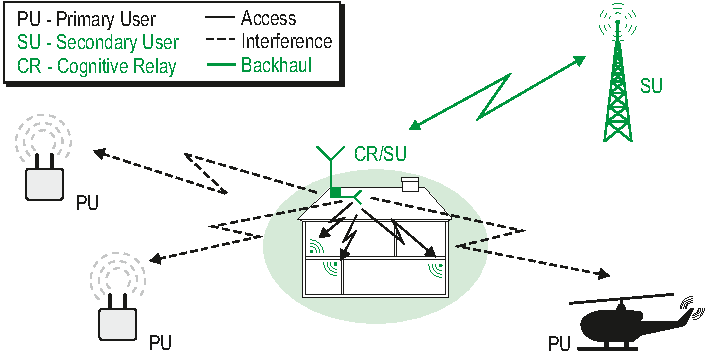
\includegraphics[trim=0.0cm 0.0cm 0.0cm 0.0cm,clip=true,width=\columnwidth]{figures/wo_channels_CR_Scenario_farbig_excess_dwl}
%        \else
%        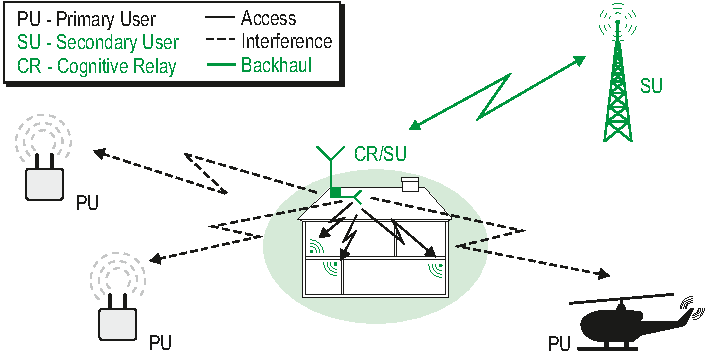
\includegraphics[trim=0.0cm 0.0cm 0.0cm 0.0cm,clip=true,width=0.5 \columnwidth]{figures/wo_channels_CR_Scenario_farbig_excess_dwl}
%        \fi
%	\makeatother
%\label{fig:ID_OC}
%	\caption{Cognitive relay downlink access.}
%	\label{fig:Cog_relay}
%\end{figure}
%\begin{figure*}[!t]
%	\centering
%	\includegraphics[trim=0.0cm 0.0cm 0.0cm 0.0cm,width=0.75\paperwidth]{figures/InterferenceScenario_Discussion20130806}
%	\caption{Modeling the interference scenario with $N$ PRs using Poisson Point Process.}
%	\label{fig:PPP_model}
%\end{figure*}

%%%%%%%%%%%%%%%%%%%%%%%%%%%%%%%%%%%%%%%%%%%%%%%%%%%%%%%%%%%%%%%%%%%%%%%%%%%%%%%%%%%%%%%%%
\section{System Model} \label{sec:sys mod}
%%%%%%%%%%%%%%%%%%%%%%%%%%%%%%%%%%%%%%%%%%%%%%%%%%%%%%%%%%%%%%%%%%%%%%%%%%%%%%%%%%%%%%%%%
\begin{figure}[!t]
        \centering
	\makeatletter
        \if@twocolumn
        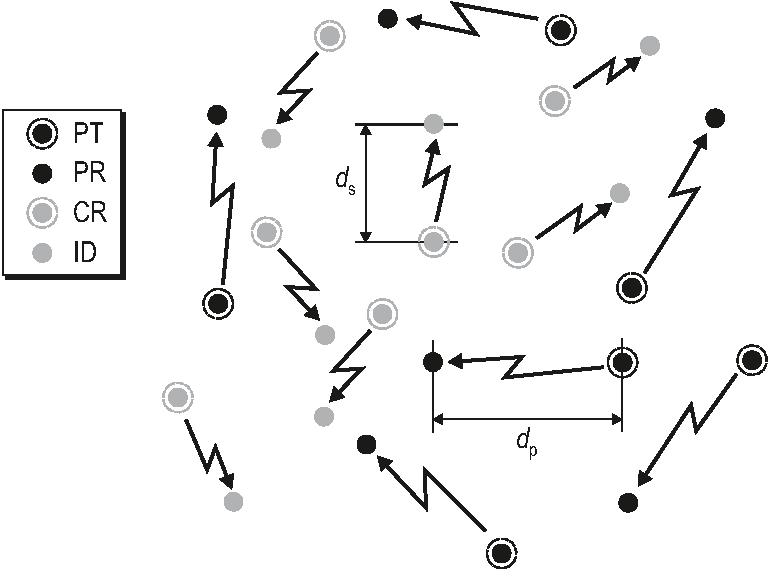
\includegraphics[trim=0.0cm 0.0cm 0.0cm 0.0cm,clip=true,width= 0.85 \columnwidth]{figures/SGeometry}
        \else
        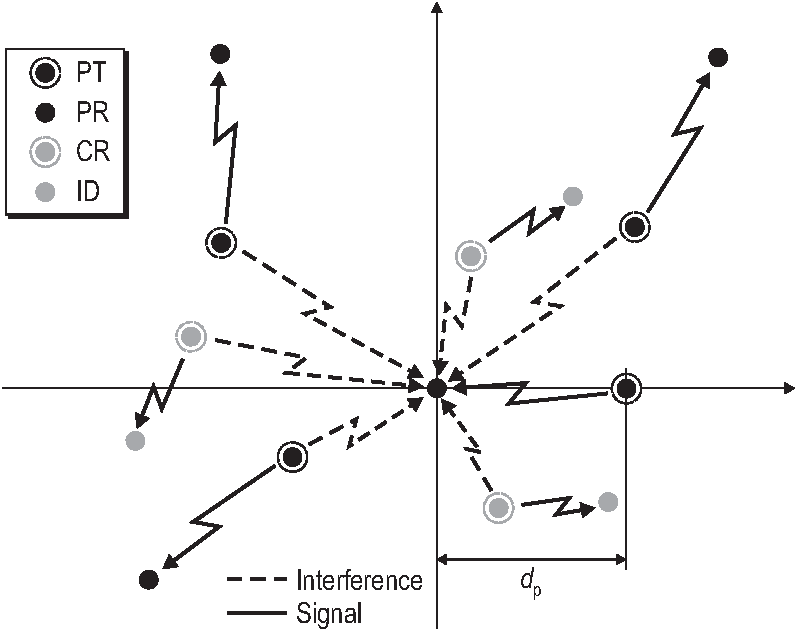
\includegraphics[trim=0.0cm 0.0cm 0.0cm 0.0cm,clip=true,width=0.5 \columnwidth]{figures/Interference_at_PR}
        \fi
	\makeatother
        \caption{A realization of a PPP for a cognitive relay network, depicting interference among the primary and secondary nodes.} %consisting of primary transmitters, primary receivers, cognitive relays as secondary transmitters and indoor devices as secondary receivers.}
	\label{fig:Int_Sc}
\end{figure}
%\subsection{Cognitive Relay}
Cognitive relay (CR) as introduced in \cite{Kaushik13, Kaushik14}, is a network element that intends to fulfill the spectral requirements of the indoor devices (IDs). 
In this paper, we extend the concept of CR as underlay system to a CRN, that is, the secondary system deploys multiple CRs and examine their effect on the primary and secondary system. For downlink transmission from CR to ID, CR and ID correspond to ST and SR. 
%CR seeks spatial reuse of the primary user spectrum. 
%All CRs forming a network are connected to secondary base station, that provides the backhaul connection. 


We assume the same transmit power for all CRs $P\sub{s}$ and preclude any form of cooperation or coordination among them. In the model, we do not involve sensing at CRs, $P\sub{s}$ can be regulated to sustain the constraint at the PR. The regulation is necessary either at the system design or at time instants where the system parameters change. With its knowledge, $P\sub{s}$ is used to characterize the capacity outage at SRs, which finally leads to a joint characterization of the OC for the CRN is determined.  
\subsection{Network Model}
%\begin{figure}[!t]
%        \centering
%	\makeatletter
%        \if@twocolumn
%        \includegraphics[trim=0.0cm 0.0cm 0.0cm 0.0cm,clip=true,width=0.7 \columnwidth]{figures/SGeometry_B}
%        \else
%        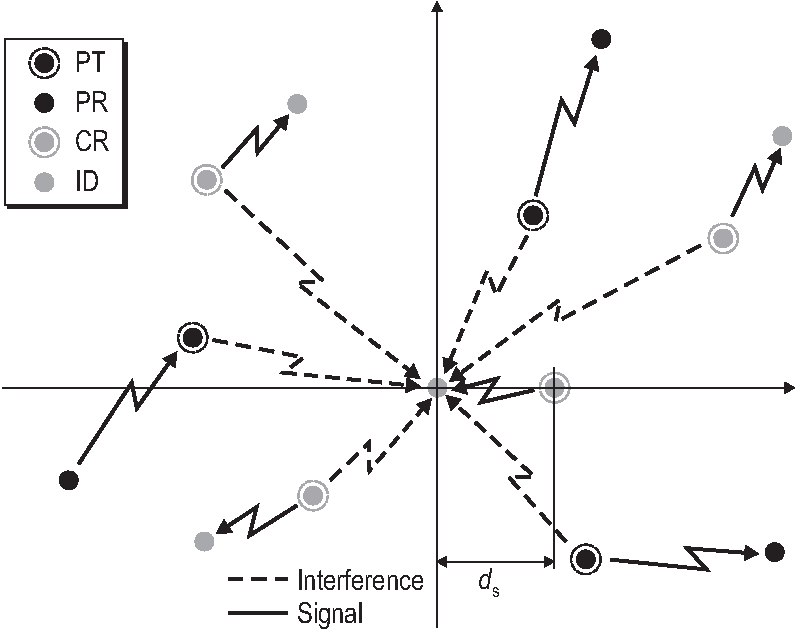
\includegraphics[trim=0.0cm 0.0cm 0.0cm 0.0cm,clip=true,width=0.5 \columnwidth]{figures/Interference_at_ID}
%        \fi
%	\makeatother
%        \caption{Interference at ID.}
%	\label{fig:Int_ID}
%\end{figure}
The locations of PTs are modelled by a stationary 2-D PPP $\Phi\sub{PT}$ of density $\lambda\sub{p}$. Similarly, the locations of CRs follow a stationary 2-D PPP $\Phi\sub{CR}$ of density $\lambda\sub{s}$, cf. \figurename~\ref{fig:Int_Sc} for an illustration. Due to the presence of transmitter-receiver pairs (PT-PR, CR-ID) in the system, the spatial distribution of PRs and IDs depends on $\Phi\sub{PT}$ and $\Phi\sub{CR}$. However, for the downlink PRs and IDs do not affect the system performance and hence do not need to be modelled. 

%Therefore, we can analyze the system based on a hypothetical PR/ID placed at an arbitrary location inside the network. %Due to stationarity of the PPP, the hypothetical PR/ID will determine the performance characteristics for other PRs/IDs in the network. 
%\\ 
%Hence, for the interference analysis, the corresponding receiver is placed at origin $o$. \\ %Same approach is also valid for the ID. \\ 
%We focus our analysis on the CR downlink performance measured at given ID at a distance $d\sub{s}$ to a given CR. Without loss of generality, we place this ID in the origin. Furthermore, the locations of primary transmitters--acting as interferers to the secondary receiver--are modelled by a PPP $\Phi_{\text{\text{PT}}}$ of density $\lambda_{\text{P}}$. Typically, primary users communicate over some target distance which introduces correlation between $\Phi_{\text{PR}}$ and $\Phi_{\text{PT}}$ that is difficult to handle analytically. We therefore propose the following two simplifying assumptions. 
%\begin{case}[Full dependence]
% ...$\Phi_{\text{\textnormal{PT}}}\equiv\Phi_{\text{\textnormal{PR}}}$
%\end{case}
%\begin{case}[No dependence]
% ...$\mathbb{P}\left(\Phi_{\text{\textnormal{PT}}}\in\cdot\,|\,\Phi_{\text{\textnormal{PR}}}\right)=\mathbb{P}\left(\Phi_{\text{\textnormal{PT}}}\in\cdot\right)$
%\end{case}
%Comment on these simplifications:
%\begin{itemize}
%	\item case full-dependence: approximation of mean distance, include figure for illustration
%	\item No-dependence: motivation: distant links, shadowing+random translation
%	\item Accuracy loss will be studied through simulations 
%\end{itemize}
%\subsection{Channel and Path Loss}
All transmitted signals are subject to a distance-dependent path loss and small-scale channel fading. The distance-dependent path loss is given as $\| \cdot \|^{-\alpha}$, where $\alpha>2$ is the path loss exponent. The small-scale channel fading is modelled as frequency-flat Rayleigh fading. Hence, the channel gains follow a unit-mean exponential distribution. The expressions presented in the paper are general and hence are applicable over a broad range of system parameters. However, to focus our analysis to the scenario described in \cite{Kaushik13}, we consider a larger transmission distance and smaller node density for the primary system compared to the secondary system, i.e., $d\sub{p} \ge d\sub{s}$ and $\lambda\sub{p} \le \lambda\sub{s}$, illustrated in \figurename~\ref{fig:Int_Sc}. %distances between the transmitter and receiver for the primary and secondary system. 
Lastly,
for a simple distinction between different scenarios, we consider that both primary and secondary systems exists either in indoor or outdoor scenario.
 This corresponds to the same $\alpha$ for the primary and secondary systems. Moreover, it is considered that larger $\alpha$, e.g., $\alpha \ge 3$ and smaller $d\sub{p}$, $d\sub{s}$ are more likely to be designated to indoor \cite{Tse05}.  
%\subsection{Medium Access}

Besides that, the primary and secondary system follow a time synchronous slotted medium access with a certain channel access probability $\beta$. Applying the independent thinning property of the PPP, the set of simultaneous active PTs again forms a homogeneous PPP with density $\beta \lambda\sub{p}$ \cite{Haenggi08now}. With no loss of generality, we consider the node density $\lambda\sub{p}$ includes the channel access probability for the PT. Similarly for CRs, $\lambda\sub{s}$ includes the channel access probability for the CR. Hence, according to this simplification, all PTs and CRs, with node densities $\lambda\sub{p}$ and $\lambda\sub{s}$, will transmit simultaneously. 
%Similarly, for the CRs with access probability $\beta\sub{s}$, the set of active CRs also forms a homogeneous PPP with density $\beta\sub{s} \lambda\sub{s}$. To simplify the analysis and with no loss of generality, we assume $\beta\sub{s} = 1$ and $\beta\sub{p} = 1$, 
%that is, in a certain time slot, all PTs and CRs perform simultaneous transmissions. Table \ref{tb:Symbol} summarizes the notation and parameters used to describe the system.   
%\subsection{Signal Model}
%\begin{itemize}
% \item Here: TDD + we consider the network in one snapshot. We have a set of primary receiver and primary transmitters  
%\end{itemize}

%\begin{figure*}[!t]
%	\centering
%	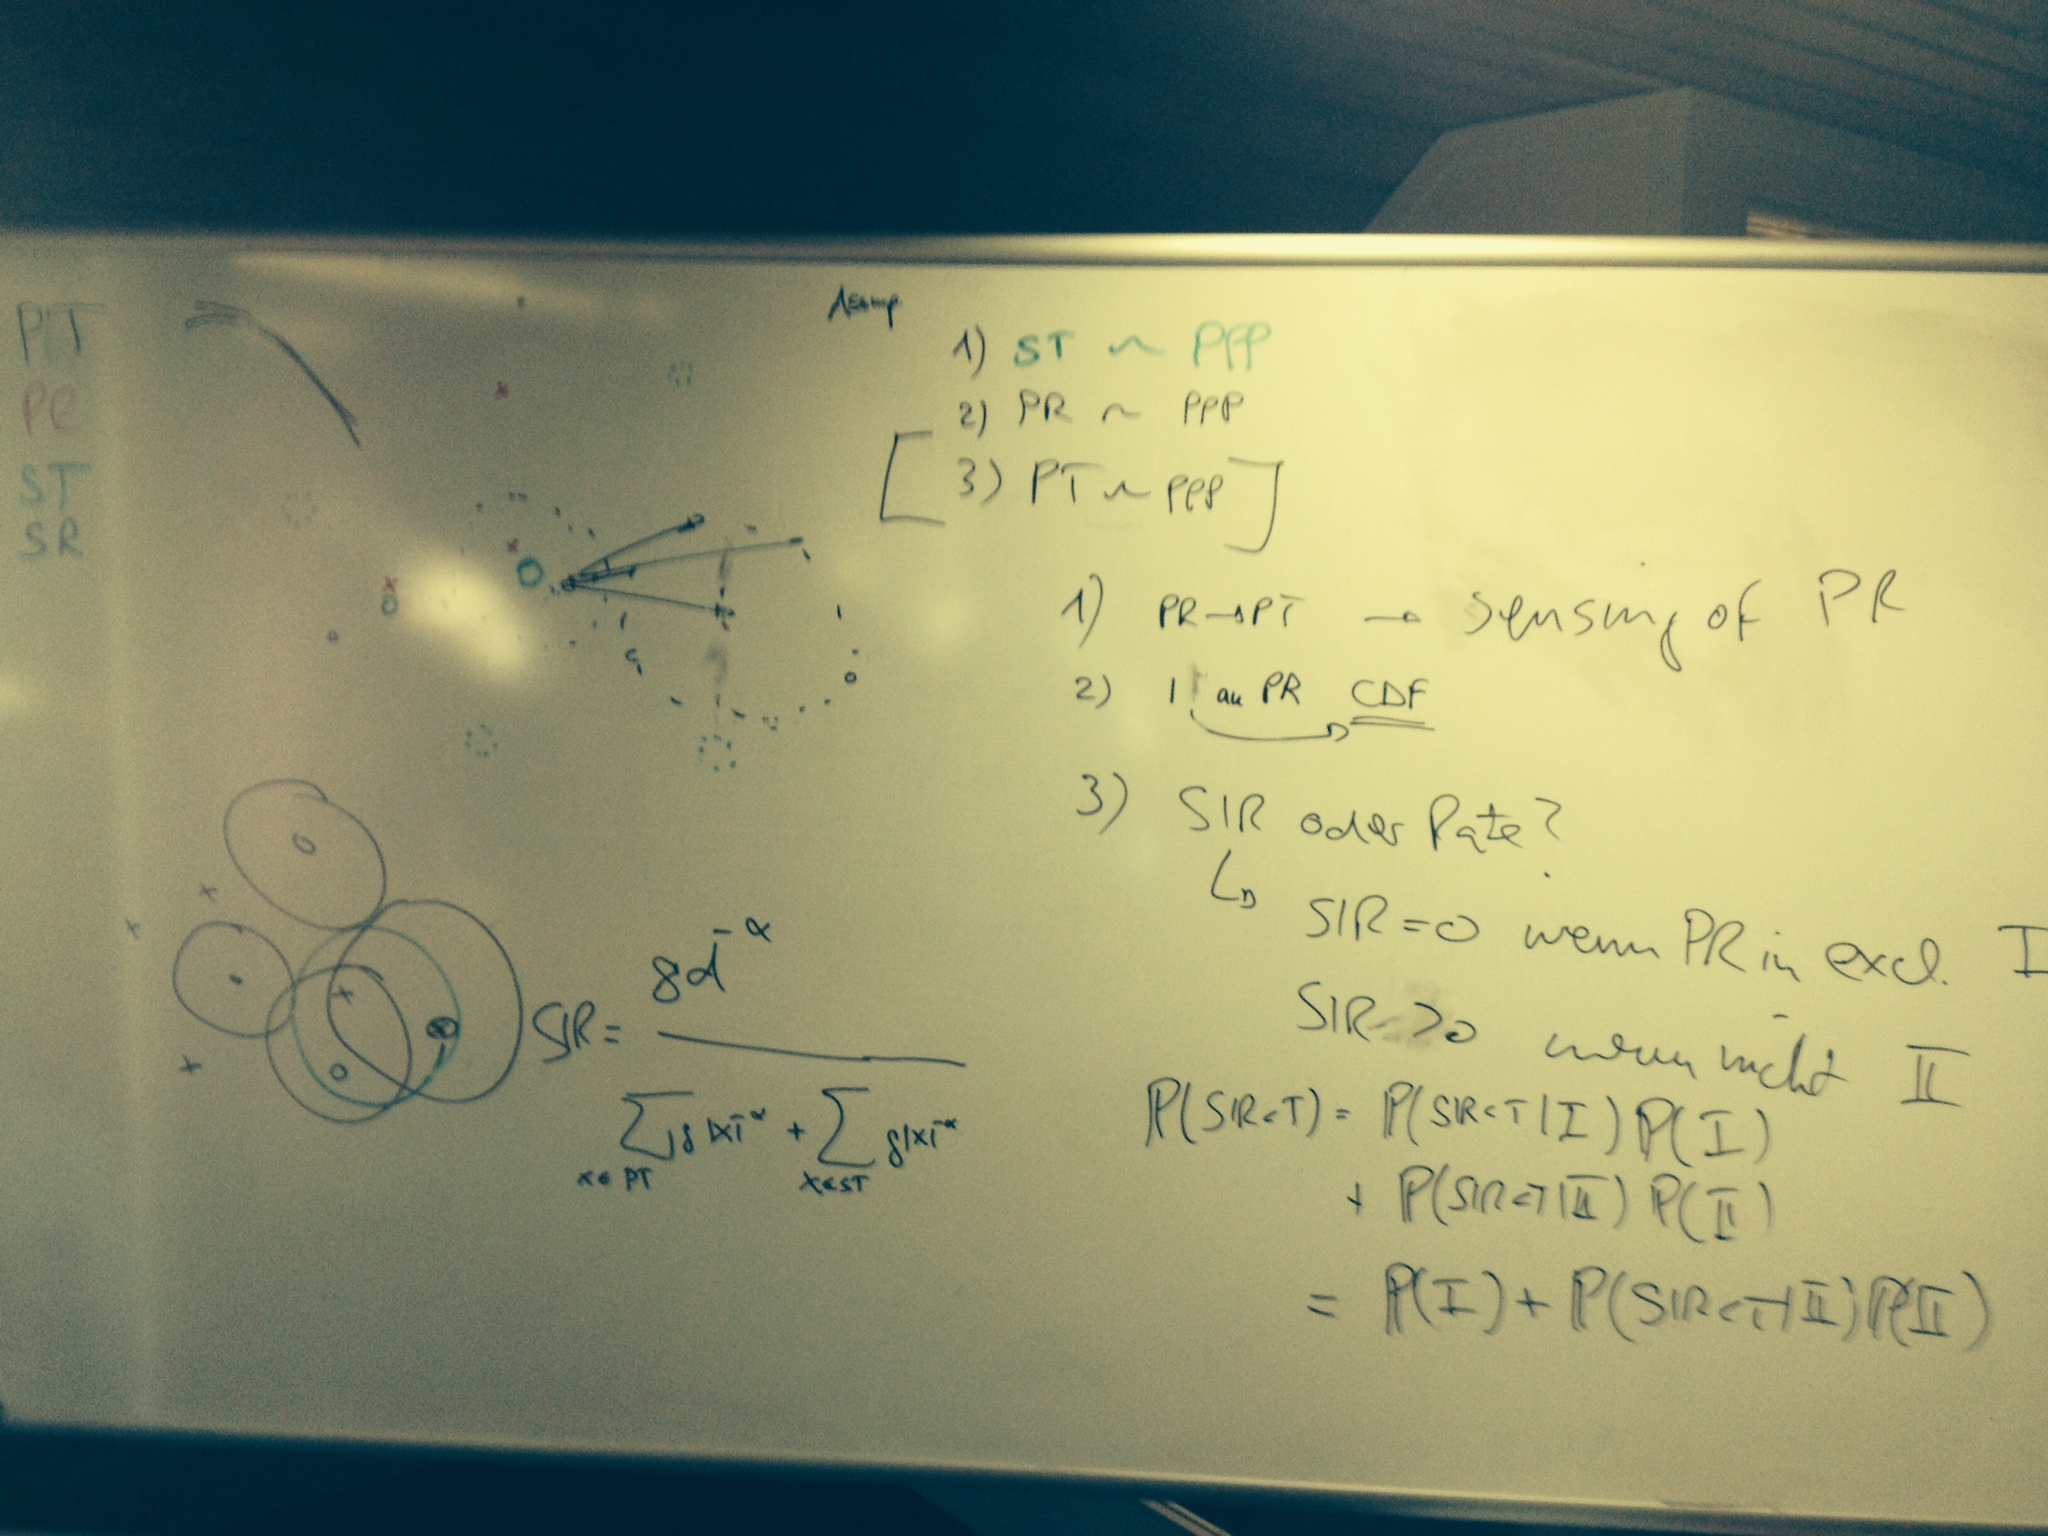
\includegraphics[trim=0.0cm 0.0cm 0.0cm 0.0cm,width=0.75\paperwidth]{figures/InterferenceScenario_Discussion20131018}
%	\caption{Modelling primary receiver and secondary receiver as PPP. The exclusion region for the cognitive relay is determined using interference temperature.}
%	\label{fig:PPP_model2}
%\end{figure*}

%\begin{figure*}[!t]
%	\centering
%	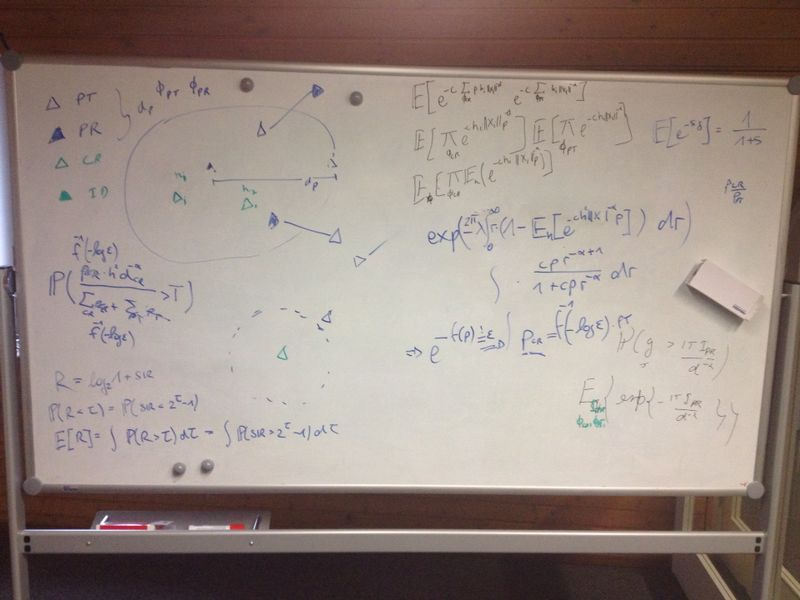
\includegraphics[trim=0.0cm 0.0cm 0.0cm 0.0cm,width=0.75\paperwidth]{figures/InterferenceScenario_Discussion20140122}
%	\caption{Modelling primary receiver and secondary receiver as PPP. Based on sharing constraints CR, CRs decide to transmit.}
%	\label{fig:PPP_model2}
%\end{figure*}
\section{Interference analysis} \label{sec:int ana}
In this section, we analyze the primary and secondary system jointly by deriving the OC. 
%Using the expression of OC, the system designer can decide whether a certain choice of parameters, the sharing constraints are satisfied or not. In the latter case, to fulfill the constraints, the secondary user parameters are adjusted to change the OC. 
To obtain an expression for the OC, we first consider the $\textsf{SIR}$ at a hypothetical PR, which we can place at origin $o$. Due to stationarity of $\Phi\sub{PT}$ and $\Phi\sub{CR}$, the $\mathsf{SIR}$ at PR is then
\begin{align}
\textsf{SIR}\sub{PR} = \frac{P\sub{p} g\sub{$o$,p} d\sub{p}^{-\alpha}}{\sum\limits_{i \in \Phi_{\text{PT}}} P\sub{p} g_i {\|X_i\|}^{-\alpha} +  \sum\limits_{j \in \Phi_{\text{CR}}} P\sub{s} g_j {\|Y_j\|}^{-\alpha}},  
\label{eq:SIR_PR}  
\end{align}
where $P\sub{p}$ and $P\sub{s}$ are the transmit power at the PT and the CR. $\|X_i\|$, $\|Y_i\|$ are the distances of the $i^{\text{th}}$ PT and $j^{\text{th}}$ CR as interferers. $g\sub{$o$,p}$, $g_i$ and $g_j$ are the channel gains for the intended PT, $i^{\text{th}}$ PT and $j^{\text{th}}$ CR as interferers. CRs must satisfy the outage constraint on $\mathsf{SIR}\sub{PR}$, given by  
\begin{equation}
\mathbb{P}(\textsf{SIR}\sub{PR} < N\sub{p}) = \text{p}\sub{out,p} \leq \epsilon\sub{p}, 
\label{eq:SIR_I}
\end{equation}
where $N\sub{p}$ and $\epsilon\sub{p}$ are the $\textsf{SIR}$ threshold and outage probability constraint at the PR. %,  defined in Table \ref{tb:Symbol}. %For the analysis, $N\sub{p} = 10$ is selected. %As already mentioned, because of stationarity of PPP, $\textsf{SIR}\sub{PR}$ characterization doesn't depend on the position of PR in the network. Hence, we position the PR at origin $o$. %%The locations of the PTs and CRs acting as interferers are modelled as $\Phi\sub{PT}$ and $\Phi\sub{CR}$ around $o$. %Because the primary and secondary systems operate independently from one another, we consider $\Phi_{\text{PT}}$ and $\Phi_{\text{CR}}$ to be independent. 
%\begin{table}
%\renewcommand{\arraystretch}{1.3}
%\caption{Symbols and Notations used}
%\label{tb:Symbol}
%\centering
%\begin{tabular}{p{0.15\columnwidth}||p{0.73\columnwidth}}
%\hline
%\bfseries Symbol & \bfseries Definition \\
%\hline\hline
%$\Phi_{\text{PT}}, \Phi\sub{CR}$ & Homogeneous PPP of the PT or CR \\ \hline
%%$\Phi_{\text{CR}}$ & Homogeneous PPP of the secondary transmitter or cognitive relay \\ \hline
%$\lambda\sub{p}, \lambda\sub{s}$ & Node density of the PT and CR\\ \hline
%%$\lambda\sub{s}$ & Node density of the cognitive relay \\ \hline
%$\|X_i\|, \|Y_j\|$ & Distances of $i^{\text{th}}$ PT and $j^{\text{th}}$ CR as interferer to origin $o$ \\ \hline 
%$g_i, g_j$ & Channel coefficients of $i^{\text{th}}$ PT and $j^{\text{th}}$ CR as interferer to origin $o$ \\ \hline
%$g_0$ & Channel coefficient of the desired PT or CR to origin $o$\\ \hline
%$P\sub{p}, P\sub{s}$ & Transmission power at PTs and CRs \\ \hline
%$d\sub{p}, d\sub{s}$ & Distance between primary and secondary transmitter-receiver pairs \\ \hline 
%%$I_{\text{th}}$ & Interference threshold at the primary receiver \\ \hline
%$N\sub{p}, N\sub{s}$ & \textsf{SIR} threshold at the PR and SR or ID \\ \hline  
%$R\sub{s}$ & Capacity threshold at the ID \\ \hline  
%$\epsilon\sub{p}$ & Outage probability constraint for \textsf{SIR} at the PR\\ \hline  
%$\psi\sub{s}$ & Outage probability constraint for capacity at the ID \\ \hline
%%$\kappa$ & Success probability for the primary network \\ \hline
%%$\beta\sub{p}, \beta\sub{s}$ & Channel access probabilities of the primary and secondary network \\ \hline
%%$\text{p}\sub{out,p}$ & Outage probability at the PR \\ \hline
%%$\text{p}\sub{out,s}$ & Outage probability at the ID \\ \hline
%\end{tabular}
%\end{table}

$\textsf{SIR}\sub{PR}$ depends on $\alpha$, primary system parameters $\lambda\sub{p}$, $P\sub{p}$ and $d\sub{p}$, as well as on the secondary system parameters $\lambda\sub{s}$ and $P\sub{s}$.
We assume that $\alpha$ and the primary system parameters are known at the system design, hence the additional interference at the PR from CRs can be regulated by choosing $P\sub{s}$ and $\lambda\sub{s}$ appropriately. 
%To evaluate the performance at the PR and the ID, two different cases are considered. In the first case, the PR is placed at origin and the intended PT is positioned at a distance $d\sub{p}$, cf. \figurename~\ref{fig:Int_Sc}, and with no loss of generality, in the second case, we replace ID at the origin and the intended CR is positioned at a distance $d\sub{s}$, refer \figurename~\ref{fig:Int_Sc}. In both cases, 
%The performance of the CRNs center around $\mathsf{SIR}\sub{PR}$ outage at PR and $\mathsf{SIR}\sub{ID}$ ouatge at ID
%CRs are allowed to transmit.
%CR senses the PRs during uplink transmission using matched filtering technique. Subjected to distance dependent path loss and Rayleigh fading, CR estimates the channel states. Thereby apply channel reciprocity principle to evaluate the received power $P_s h_i {||X_i||^{-\alpha}}$ at the $i^{\text{th}}$ PR, where $i \in \Phi_{\text{PR}}$. \\
%CR encounters a transmission opportunity when the power received at PR is below interference threshold $I_{\text{th}}$, written as
%CRs are allowed to transmit with a constant transmit power $P_s$ when
%\begin{align}
%\mathbb{P}(\textsf{SIR} > N_{\text{SIR}})
%\maxi_{i \in \Phi_{\text{PR}}}  \{ P_s h_i {||X_i||^{-\alpha}} \} <  I_{\text{th}}.
%\end{align} 
%Excluding the secondary system, the performance of the primary system can be characterized through the success probabilty $\kappa$. 

Before proceeding further, it is useful to characterize the performance of the system at the PR with only PTs as interferers. 
\begin{lemma}\label{lem:lemma1}
\normalfont
The success probability for a PR in absence of CRs is given by\cite[(3.29)]{Haenggi08now}
\begin{align}
\kappa = \p \left( \frac{P\sub{p} g\sub{$o$,p} d\sub{p}^{-\alpha}}{\sum\limits_{i \in \Phi_{\text{PT}}} P\sub{p} g_i {\|X_i\|}^{-\alpha}}  > N\sub{p} \right)  = \exp \left( - \frac{2 \pi^2 \lambda_{\text{p}}  {c_1}^\frac{2}{\alpha}}{\alpha \sin \left( \frac{2 \pi}{\alpha}\right)} \right), 
\label{eq:lem1}
\end{align}  
where $c_1 = N\sub{p} d\sub{p}^{\alpha}$. %$g\sub{$o$,p}$ represents the channel gain for the intended PT to PR. $g_i$ is the channel gain for the $i^{\text{th}}$ PT as interferer at a distance $\|X_i\|$ to the PR at $o$.
\end{lemma} 
\begin{remark} \label{rem:rem1}
\normalfont
$\kappa$ decreases exponentially with increase in $d\sub{p}$, $\lambda\sub{p}$ and $N\sub{p}$. Moreover, $\alpha \sin\left( 2 \pi/\alpha \right)$ is increasing and $N\sub{p}^{2/\alpha}$ is decreasing with $\alpha$, where $N\sub{p} > 1$, hence $\kappa$ increases with $\alpha$. 
\end{remark}
%\begin{lemma}\label{lem:lemma2}
%\normalfont
%For an exponentially distributed channel coefficient $\mathsf{g}$\cite[(3.21)]{Haenggi08now} 
%\begin{equation}
%\e{\mathsf{g}}{\int\limits_{0}^{\infty} 2r \left( 1 - e^{ - c g r^{-\alpha} } \right) dr} = c^{\frac{2}{\alpha }} \frac{\frac{ 2 \pi}{\alpha}}{\sin \left( \frac{2 \pi}{\alpha}\right)}
%\label{eq:lem2}
%\end{equation}  
%\end{lemma}

With the inclusion of CRs, the success probability $1 - p\sub{out,p}$ and subsequently the constraint $1 - \epsilon\sub{p} $ at PR is limited by $\kappa$, hence $\kappa \ge 1 - \epsilon\sub{p}$. Therefore, it makes sense to account for the degradation in the primary system performance relative to $\kappa$. 
\begin{prop} \label{prop:prop1}
\normalfont
The relative degradation of the success probability at PR is given by 
\begin{equation}
\theta = \frac{1 - \epsilon\sub{p}}{\kappa}, 
\label{eq:prop1}
\end{equation}
where $0 \le \theta \le 1$. For example, $\theta  = 0.95$ represents $5\%$ degradation in success probability $\kappa$. 
\end{prop}

As discussed, all CRs transmit simultaneously with $P\sub{s}$. For a certain node density $\lambda\sub{s}$ and $\theta$, as per the system requirement it is important to determine the maximum transmit power $P\sub{s}$ at CRs, such that the constraint in (\ref{eq:SIR_I}) is satisfied. 
\begin{lemma}\label{lem:lemma2}
\normalfont 
For sustaining (\ref{eq:SIR_I}), the maximum transmit power $P\sub{s}$ at CRs is 
\begin{align}
P\sub{s} \le \frac{P\sub{p}}{N\sub{p}} \left( \frac{\alpha \sin \left( \frac{2 \pi}{\alpha} \right)}{2 \pi^2 \lambda\sub{s} d\sub{p}^{2}  } \ln \left( \frac{\kappa}{1 - \epsilon\sub{p}} \right) \right)^{\frac{\alpha}{2}}.
\label{eq:tpCR}
\end{align} 
\end{lemma}
\begin{IEEEproof}
To solve for $P\sub{s}$, we consider the constraint in (\ref{eq:SIR_I}) 
\begin{align}
\epsilon_{\text{p}} \gthan{\text{}}& \p \left( \textsf{SIR}\sub{PR}  < N\sub{p} \right) \nonumber \\ 
%\epsilon_{\text{p}} \gthan{\text{}}& \p \left( \frac{P\sub{p} g_0 d\sub{p}^{-\alpha}}{\sum\limits_{i \in \Phi_{\text{PT}}} P\sub{p} g_i {\|X_i\|}^{-\alpha} +  \sum\limits_{j \in \Phi_{\text{CR}}} P\sub{s} g_j {\|Y_j\|}^{-\alpha}} < N\sub{p} \right) \label{eq:SIR_PR} \\ 
\quad \eqto^{(a)}& \p \left( g\sub{$o$,p} < \frac{\sum\limits_{i \in \Phi_{\text{PT}}} N\sub{p} g_i {\|X_i\|}^{-\alpha} +  \sum\limits_{j \in \Phi_{\text{CR}}} \gamma N\sub{p} g_j {\|Y_j\|}^{-\alpha}}{d\sub{p}^{-\alpha}} \right) \nonumber \\ 
\quad \eqto^{(b)}& 1 - \e{\mathsf{}}{\exp \left(- \frac{\sum\limits_{i \in \Phi_{\text{PT}}} N\sub{p} g_i {\|X_i\|}^{-\alpha} +  \sum\limits_{j \in \Phi_{\text{CR}}} \gamma N\sub{p} g_j {\|Y_j\|}^{-\alpha}}{d\sub{p}^{-\alpha}}  \right)} \nonumber \\
\quad \eqto^{(c)}& 1 - \e{ \Phi_{\text{PT}} } {\e{g} { \prod\limits_{i \in \Phi_{\text{PT}}} \exp\left(- \frac{N\sub{p} g_i {\|X_i\|}^{-\alpha}}{d\sub{p}^{-\alpha}} \right) } } \nonumber \\ 
\quad & \times \e{ \Phi_{\text{CR}} } { \e{g} { \prod\limits_{j \in \Phi_{\text{CR}}} \exp \left( - \frac{\gamma N\sub{p} g_j {\|Y_j\|}^{-\alpha}}{d\sub{p}^{-\alpha}} \right) }} \nonumber \\ 
%\quad \eqto^{(d)}& 1 - \smash[b]{\underbrace{\exp \left( - \pi \beta\sub{p} \lambda_{\text{p}} \e{\mathsf{g}}{\int\limits_{0}^{\infty} 2r \left( 1 - e^{ - c_1 g r^{-\alpha} } \right) dr} \right)}_{E_1}} \cdot \nonumber \\[2.5em] 
%\quad & \exp \left( -\pi \beta\sub{s} \lambda_{\text{s}} \smash[b]{\underbrace{\e{\mathsf{g}}{\int\limits_{0}^{\infty} 2r \left( 1 - e^{ - c_2 g r^{-\alpha} } \right) dr }}_{E_2}} \right) \nonumber \\[1.5em]
\quad \eqto^{(d)}& 1 - \kappa \cdot \smash[b]{\underbrace{\exp \left( - 2\pi^2 \frac{c_2^{\frac{2}{\alpha}} \lambda\sub{s}}{\alpha \sin \left( \frac{2\pi}{\alpha} \right)} \right)}_{\theta}} \label{eq:SIROutPR}   
%\quad \gthan^{(e)}& 1 - \exp \left( -2 \pi \lambda_{\text{PT}} \int\limits_{0}^{\infty} \left( \frac{c_1r}{c_1 + r^{\alpha}} \right) dr \right) \cdot \exp \left( -2 \pi \lambda_{\text{CR}} \int\limits_{0}^{\infty} \left( \frac{c_2r}{c_2 + r^{\alpha}} \right) dr \right) \cdot \nonumber \\
%\quad \gthan^{(f)}& 1 - \exp \left( -2 \pi \lambda_{\text{PT}} \left. \frac{\sqrt{c_1}}{2} \arctan{\frac{r^2}{\sqrt{c_1}}} \right|_{r=0}^{\infty} \right) \cdot \exp \left( -2 \pi \lambda_{\text{CR}} \left. \frac{\sqrt{c_2}}{2} \arctan{\frac{r^2}{\sqrt{c_2}}} \right|_{r=0}^{\infty} \right) \nonumber
\end{align}
\\[0.5em]
where $c_2 = \gamma N\sub{p} d\sub{p}^{\alpha}$. (a) defines $\gamma = P\sub{s}/P\sub{p}$, $(b)$ represents the expectation operation $\e{\mathsf{}}{}$ over $\Phi_{\text{PT}}$, $\Phi_{\text{CR}}$, $g_i$ and $g_j$. $(c)$ follows from the independence between $\Phi_{\text{PT}}$ and $\Phi_{\text{CR}}$. $\e{g}{}$ represents the expectation over channel gains for the nodes corresponding to either $\Phi\sub{PT}$ or $\Phi\sub{CR}$. Moreover, $(c)$ uses the probability generating functional (PGFL) \cite[Appendix, A.5]{Haenggi08now} and (\ref{eq:lem1}) to obtain $(d)$. 
%$(e)$ replaces $\e{\mathsf{g}}{}$ with the Laplace transform of the exponential distribution $\e{\mathsf{g}}{e^{-sg}} = \frac{1}{1+s}$ and 
%It further substitutes $c_1 = N\sub{p} d\sub{p}^{\alpha}$ and $c_2 = \gamma N\sub{p} d\sub{p}^{\alpha}$.%, and $(e)$ uses (\ref{eq:lem1}),\cite[(3.21)]{Haenggi08now} to replace expressions $E_1$ and $E_2$.
\end{IEEEproof}

\begin{figure}[!t]
\centering
\begin{tikzpicture}[scale=1]
\node[anchor=south west,inner sep=0] (image) at (0,0)
{
\makeatletter
\if@twocolumn
	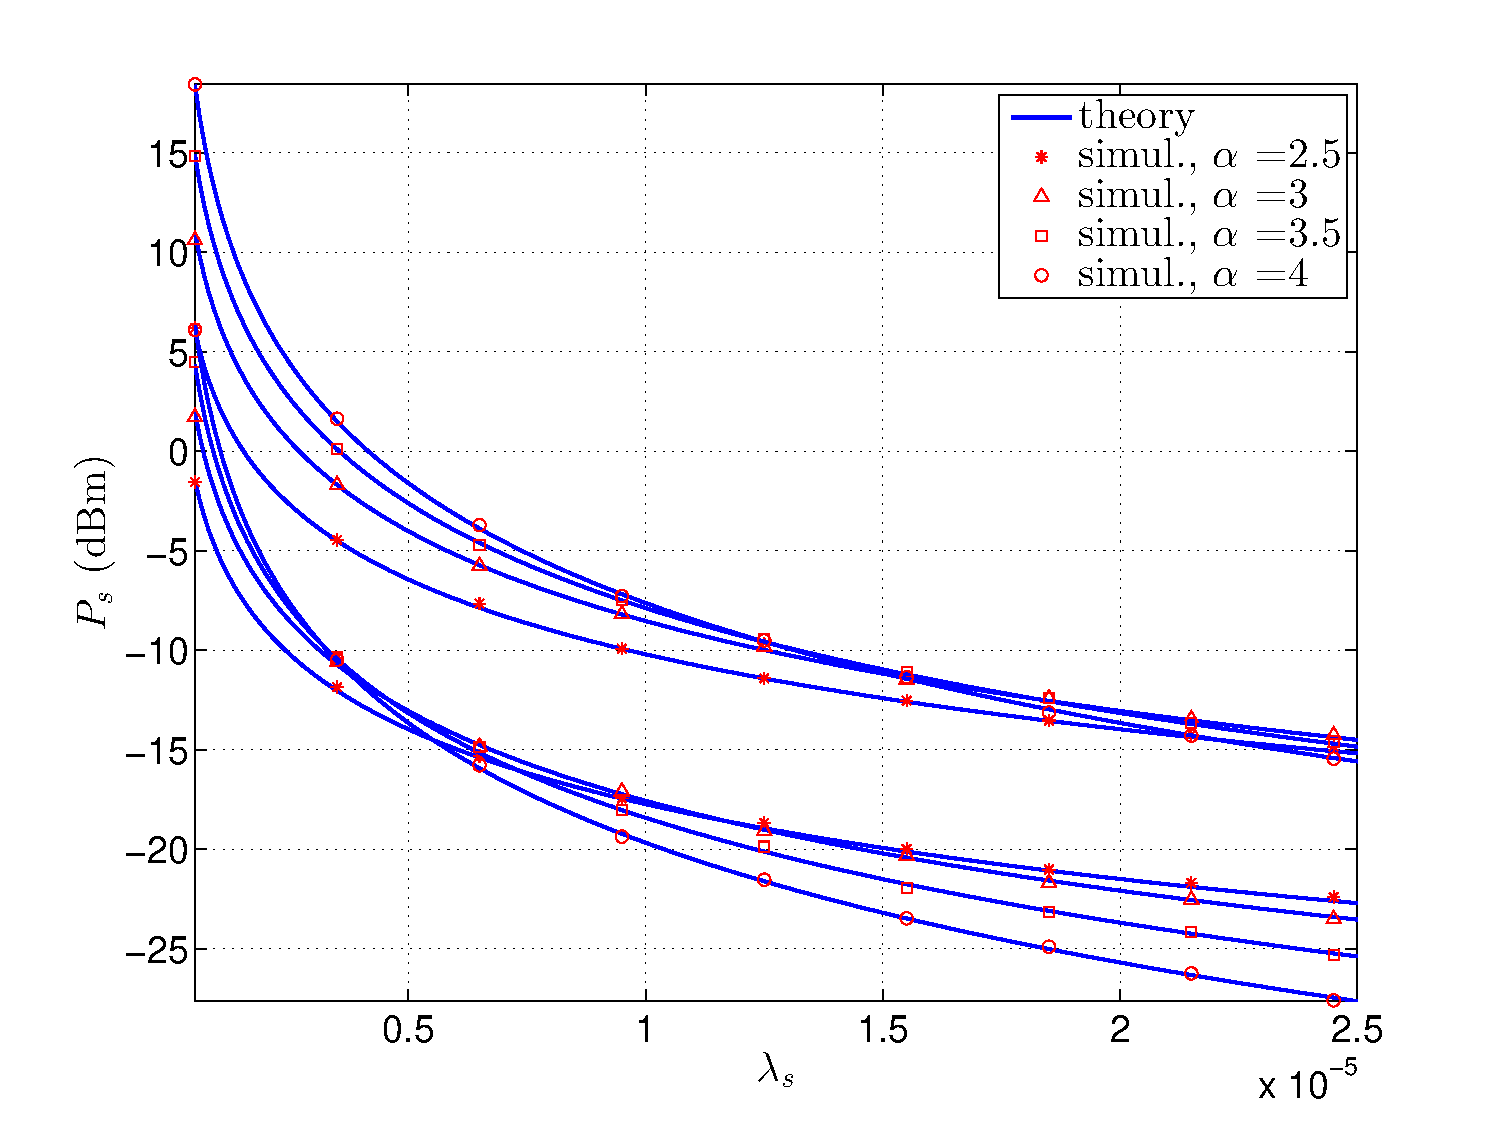
\includegraphics[trim=1.2cm 0.4cm 1.6cm 1.2cm,clip=true,width=\columnwidth]{figures/fig_CR_Txp_vs_lambda_CR_wkr_1e5}
\else
	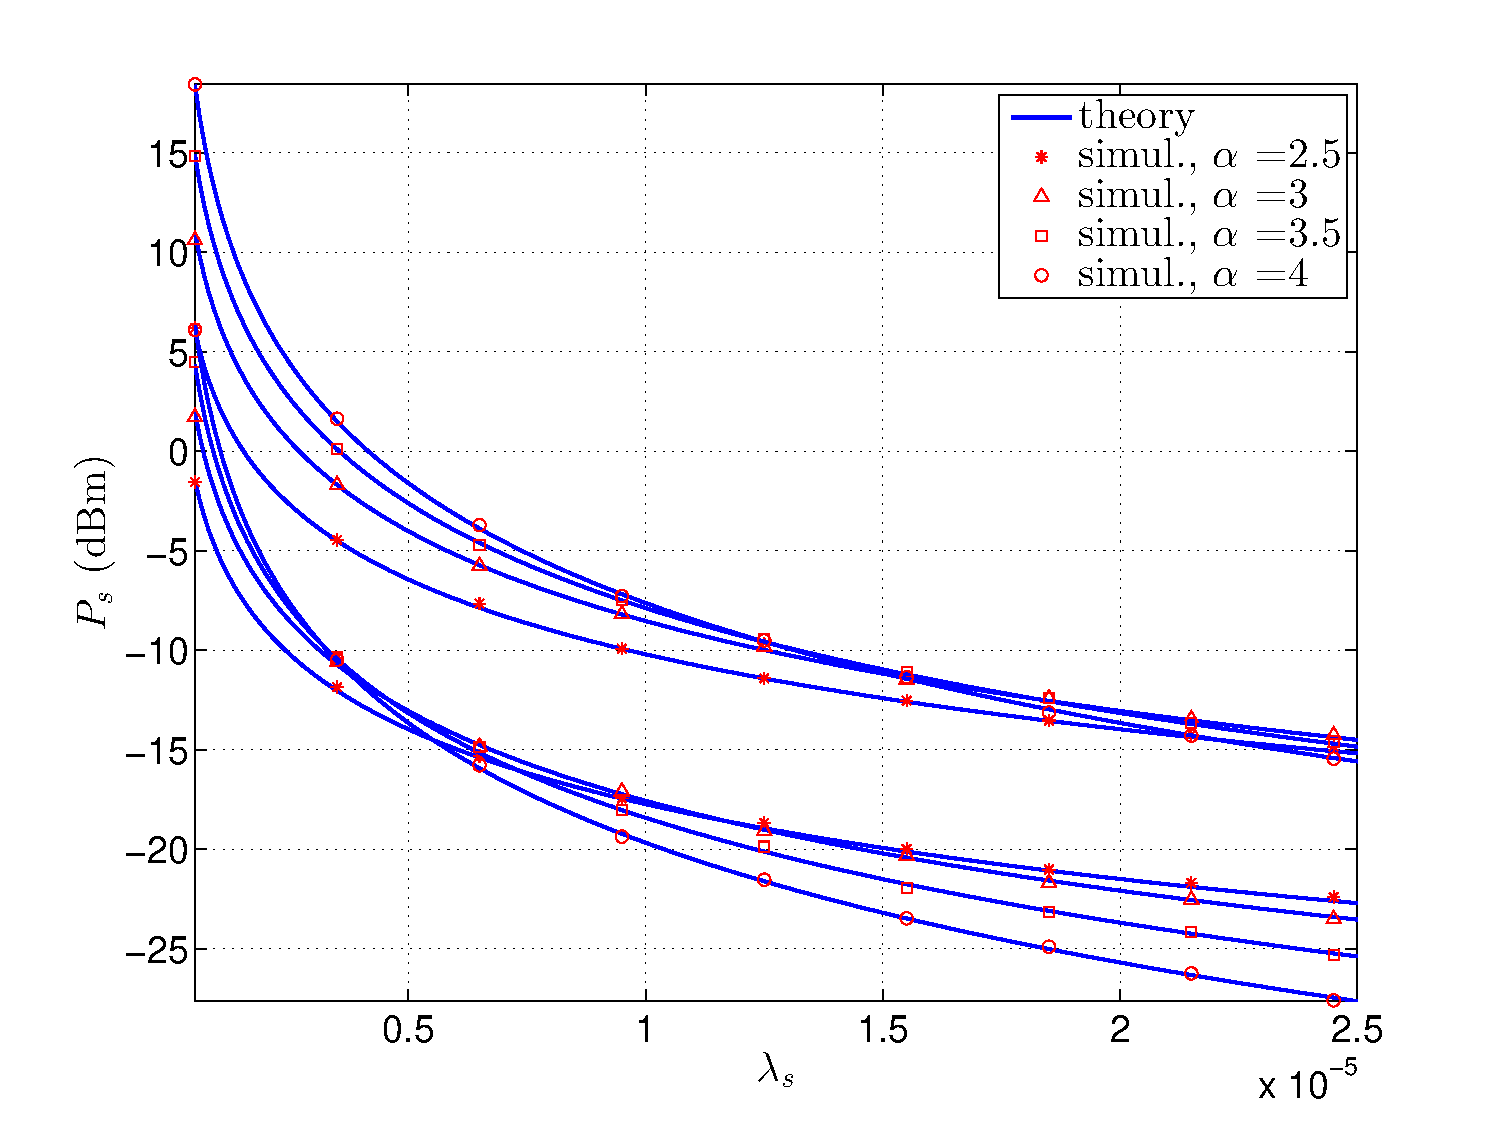
\includegraphics[trim=0.0cm 0.0cm 0.0cm 0.0cm,clip=true,width=0.5 \columnwidth]{figures/fig_CR_Txp_vs_lambda_CR_wkr_1e5}
\fi
\makeatother
};
\begin{scope}[x={(image.south east)},y={(image.north west)}]
%\draw  (0.832,0.99) node[above=-0.1pt, font=\small] {$I_{\text{th}}$};
%\draw  (.97,0.898) node[right=-2.2pt, font=\small] {$\epsilon_{\text{I,out}}$};
%\draw[black,thick,<->] (0.97,0.898) --  node[right=-2.2pt, font=\small] {$\epsilon_{\text{I,out}}$} (0.97,0.985);
%\draw [thick] (0.831,0.985) -- (0.831,0.096);
%\draw [thick] (0.08,0.898) -- (0.956,0.898);

% Select curves depending upon theta   
\draw (0.65,0.17) arc(-130:130:0.7mm and 3.05mm)  node[above=0.35mm, font=\tiny] {$d_{\text{p}}$ = 100};
\draw (0.33,0.47) arc(-130:130:0.7mm and 3.05mm)  node[above=0.35mm, font=\tiny] {$d\sub{p}$ = 50};
\draw[black,->] (0.2,0.52) --  node[above=4.2mm,right=2.1mm, font=\tiny] {$\alpha$} (0.27,0.62);
\draw[black,->] (0.815,0.22) --  node[above=4.2mm,right=2.1mm, font=\tiny] {$\alpha$} (0.745,0.12);

%\draw[help lines,xstep=.1,ystep=.1] (0,0) grid (1,1);
%\foreach \x in {0,1,...,9} { \node [anchor=north] at (\x/10,0) {0.\x}; }
%\foreach \y in {0,1,...,9} { \node [anchor=east] at (0,\y/10) {0.\y}; }
\end{scope}
\end{tikzpicture}
\caption{Maximum transmit power of CRs for a given node density $\lambda\sub{s}$, with different choices of $d\sub{p}$ and $\alpha$, where $\theta = 0.95$, $N\sub{p} = \SI{10}{}$, $P\sub{p} = \SI{10}{dBm}$ and $\lambda\sub{p} = 10^{-6} \text{nodes}/{\text{m}^2}$.} 
\label{fig:tpCR}
\end{figure}
\begin{remark} \label{rem:rem2}
\normalfont
(\ref{eq:SIROutPR}) represents the $\textsf{SIR}\sub{PR}$ outage probability $p\sub{out,p}$. Similar to $\kappa$ in Remark \ref{rem:rem1}, $\theta$ increases with $\alpha$ and decreases with $d\sub{p}$. Hence, better performance, that is lower $p\sub{out,p}$ at PR is obtained for the scenarios with larger $\alpha$ and smaller $d\sub{p}$.
Now, $P\sub{s}$ in Lemma \ref{lem:lemm3}, obtained from our system model, can serve as a LPB for other systems with more sophisticated intereference coordination that involves sensing. From (\ref{eq:tpCR}), it is clearly observed that $P\sub{s}$ increases proportionally to $P\sub{p}$, and inversely to $N\sub{p}$. Moreover $\alpha/2 > 1$, thus, for fixed $\alpha$, $P\sub{s}$ decreases exponentially with $d\sub{p}$ and $\lambda\sub{s}$. It is worth noting that, $P\sub{s}$ increases exponentially with $\ln \left( \kappa/1- \epsilon\sub{p} \right) = \ln\left( 1/\theta\right)$, cf. (\ref{eq:prop1}). 
%\begin{equation}
%P\sub{s} = 
%\begin{cases} 
%\text{increases exponentially with $\log\left( \frac{1}{1 - \theta} \right)$} & \mbox{if $\theta > 1 - \frac{1}{e}$} \\
%\text{decreases exponentially with $\log\left( \frac{1}{1 - \theta} \right)$} & \mbox{if $\theta < 1 - \frac{1}{e}$} \\
%\text{constant with $\log\left( \frac{1}{1 - \theta} \right)$} & \mbox{if $\theta = 1 - \frac{1}{e}$} \\
%\end{cases}
%\end{equation}
Although $\alpha \sin\left( 2\pi/\alpha \right)$ is increasing with $\alpha$, still $P\sub{s}$ is non-monotonic with $\alpha$, see \figurename~\ref{fig:tpCR}. 
%due to the expression $(\cdot )^{\frac{\alpha}{2}}$, cf. (\ref{eq:tpCR}). 
That is, for operation point 1, where $\lambda\sub{s} = 2 \cdot 10^{-5}$ and $d\sub{p}=100$, larger $\alpha$ degrades the signal power more than the interference from PTs and CRs. Hence to sustain a constant degradation $\theta = 0.95$, CRs must operate at relatively lower $P\sub{s}$ to satisfy (\ref{eq:SIR_I}), and vice versa for operation point 2, where $\lambda\sub{s} = 1 \cdot 10^{-5}$ and $d\sub{p} = 50$. Hence, for a constant $\theta$, the effect of $\alpha$ is compensated by regulating $P\sub{s}$ at CRs. 
\end{remark}

We now investigate the performance at the ID. The $\textsf{SIR}$ at a hypothetical ID is 
\begin{equation}
\mathsf{SIR}\sub{ID} = \frac{P\sub{s} g\sub{$o$,s} d\sub{s}^{-\alpha}}{\sum\limits_{i \in \Phi_{\text{PT}}} P\sub{p} g_i {\|X_i\|}^{-\alpha} +  \sum\limits_{j \in \Phi_{\text{CR}}} P\sub{s} g_j {\|Y_j\|}^{-\alpha}}.
\label{eq:SIR_ID}  
\end{equation}
Analogous to (\ref{eq:SIR_PR}), due to stationarity of $\Phi\sub{PT}$ and $\Phi\sub{CR}$, the hypothetical ID is placed at $o$. $g\sub{$o$,s}$ represents the channel gain for the intended CR to ID at a distance $d\sub{s}$. Moreover, from $\textsf{SIR}\sub{ID}$ the capacity at the ID is determined as 
\begin{equation}
\textsf{C}\sub{ID} = \log_2 (1 + \textsf{SIR}\sub{ID}).
\label{eq:Cap}
\end{equation} 
Hence, the performance of the secondary system can be determined from the $\mathsf{SIR}\sub{ID}$ outage probability 
\begin{align}
\mathbb{P}(\textsf{SIR}\sub{ID} < N\sub{s}) &= \text{p}\sub{out,s} \label{eq:SIR_Out} \\
\intertext{or equivalently, from the $\textsf{C}\sub{ID}$ outage probability} 
\mathbb{P}(\textsf{C}\sub{ID} < R\sub{s}), \label{eq:Cap_Out}
\end{align} 
where $N\sub{s}$ and $R\sub{s}$ are the \textsf{SIR} and rate threshold at ID. 
%Similar to PR, now we place the reference ID at $o$. 
Again, $\mathsf{SIR}\sub{ID}$ depends on the system parameters $P\sub{p}$, $\lambda\sub{p}$ and $d\sub{p}$ and $\alpha$, which are assumed to be known as well as on the parameters $\lambda\sub{s}$, $d\sub{s}$ and $P\sub{s}$, which can be regulated by system designer. %$P\sub{s}$ determined in Lemma \ref{lem:lemma2} is substituted in (\ref{eq:SIR_ID}) to include $\epsilon\sub{p}$ in the expression and obtain the OC for the system. 
\begin{lemma}\label{lem:lemm3}
\normalfont 
The $\mathsf{SIR}\sub{ID}$ outage probability for ID in the CRN is given by 
\begin{align}
p\sub{out,s} = 1 - \left(1 - \epsilon{\sub{p}}\right)^{N\sub{s}^{\frac{2}{\alpha}} m}, 
\label{eq:SIROutID}
\end{align}
where 
\begin{equation}
m = \frac{2 \pi^2 \lambda\sub{s}d\sub{s}^2}{ \alpha \sin\left( \frac{2\pi}{\alpha} \right) \ln \left( \frac{\kappa}{1 - \epsilon\sub{p}} \right) }.
\label{eq:m}
\end{equation}
%$\kappa$ and $\epsilon\sub{p}$ are given in (\ref{eq:lem1}) and (\ref{eq:tpCR}), and $m = \frac{2 \pi^2 \lambda\sub{s}d\sub{s}^2}{ \alpha \sin\left( \frac{2\pi}{\alpha} \right) \ln \left( \frac{\kappa}{1 - \epsilon\sub{p}} \right) }$. 
\end{lemma}
\begin{IEEEproof}
The outage probability of $\mathsf{SIR}_{\text{ID}}$ is evaluated as
\begin{align}
p\sub{out,s} =& \p(\mathsf{SIR}_{\text{ID}} < N\sub{s}) \nonumber \\ 
%		 \overset{\text{ }}{=}& \p(\mathsf{SIR}_{\text{ID}} < N\sub{s} ) \nonumber \\ 
%		 =& \p \left( \frac{\text{P}_s g_0 d_s^{-\alpha}}{\sum\limits_{i \in \Phi_{\text{PT}}} \text{P}_p g_i {\|X_i\|}^{-\alpha} +  \sum\limits_{j \in \Phi_{\text{CR}}} \text{P}_s g_j {\|Y_j\|}^{-\alpha}} < N\sub{s} \right) \label{eq:SIR_ID} 
\quad \overset{(a)}{=}& 1 - \exp \left( - 2\pi^2 \frac{c_3^{\frac{2}{\alpha}} \lambda\sub{p}}{\alpha \sin \left( \frac{2\pi}{\alpha} \right)} \right) \exp \left( - 2\pi^2 \frac{c_4^{\frac{2}{\alpha}} \lambda\sub{s}}{\alpha \sin \left( \frac{2\pi}{\alpha} \right)} \right) \nonumber \\   
\quad \overset{(b)}{=}& 1 - \kappa^{\left[ \left(  \frac{c_3}{c_1}\right)^{\frac{2}{\alpha}}\right] } \cdot \theta^{\left[ \left(  \frac{c_4}{c_2}\right)^{\frac{2}{\alpha}}\right] } \nonumber \\ 
\quad \overset{(c)}{=}& 1 - \left( \kappa \cdot \theta \right) ^{ \left[ \left(  \frac{P\sub{p} N\sub{s} d\sub{s}^{\alpha}}{P\sub{s} N\sub{p} d\sub{p}^{\alpha}} \right)^{\frac{2}{\alpha}} \right] } \nonumber 
%\quad \overset{(b)}{=}& 1 - \left[ \smash[b]{\underbrace{\exp \left( - 2\pi^2 \frac{c_1^{\frac{2}{\alpha}} \lambda\sub{p}}{\alpha \sin \left( \frac{2\pi}{\alpha} \right)} \right)}_{\kappa}} \right]^{\left(  \frac{c_3}{c_1}\right)^{\frac{2}{\alpha}}} \times \nonumber \\[.8em] 
%\quad & \left[ \smash[b]{\underbrace{\exp \left( - 2\pi^2 \frac{c_2^{\frac{2}{\alpha}} \lambda\sub{s}}{\alpha \sin \left( \frac{2\pi}{\alpha} \right)} \right)}_{\omega}} \right]^{\left(  \frac{c_4}{c_2}\right)^{\frac{2}{\alpha}}} \nonumber \\[.0em] \nonumber 
%\quad \overset{(c)}{=}& 1 - \left[ \kappa \right]^{\left(  \frac{c_3}{c_1}\right)^{\frac{2}{\alpha}}} \left[ 1- \theta \right]^{\left(  \frac{c_4}{c_2}\right)^{\frac{2}{\alpha}}} \nonumber  
\end{align}
where $c_3 = (1/\gamma) N\sub{s} d\sub{s}^{\alpha}$ and $c_4 = N\sub{s} d\sub{s}^{\alpha}$. (a) follows the same procedure as in the proof of Lemma \ref{lem:lemma2}, (b) uses $e^{ab} = \left[e^{a}\right]^{b}$ and $(c)$ substitutes $P\sub{s}$ from (\ref{eq:tpCR}) to obtain the final expression. 
\end{IEEEproof}
Substituting the expressions from (\ref{eq:Cap}), (\ref{eq:SIR_Out}), (\ref{eq:Cap_Out}) inside (\ref{eq:SIROutID}) in Lemma \ref{lem:lemm3} to derive OC for the CRN. 
\begin{theorem} \label{th:theo1}
\normalfont
The operating characteristics for the CRN are given by  
\begin{align}
\psi\sub{s} \ge \p(\mathsf{C}_{\text{ID}} < R\sub{s}) = 1 - \left(1 - \epsilon{\sub{p}}\right)^{ \left( 2^{R\sub{s}}-1 \right)^{\frac{2}{\alpha}} m }, 
\label{eq:OC} 
\end{align}
where $\psi\sub{s}$ is the outage probability constraint on the $\textsf{C}\sub{ID}$ outage probability given by (\ref{eq:Cap_Out}). 
\end{theorem}
\begin{figure}[!t]
\makeatletter
\if@twocolumn
        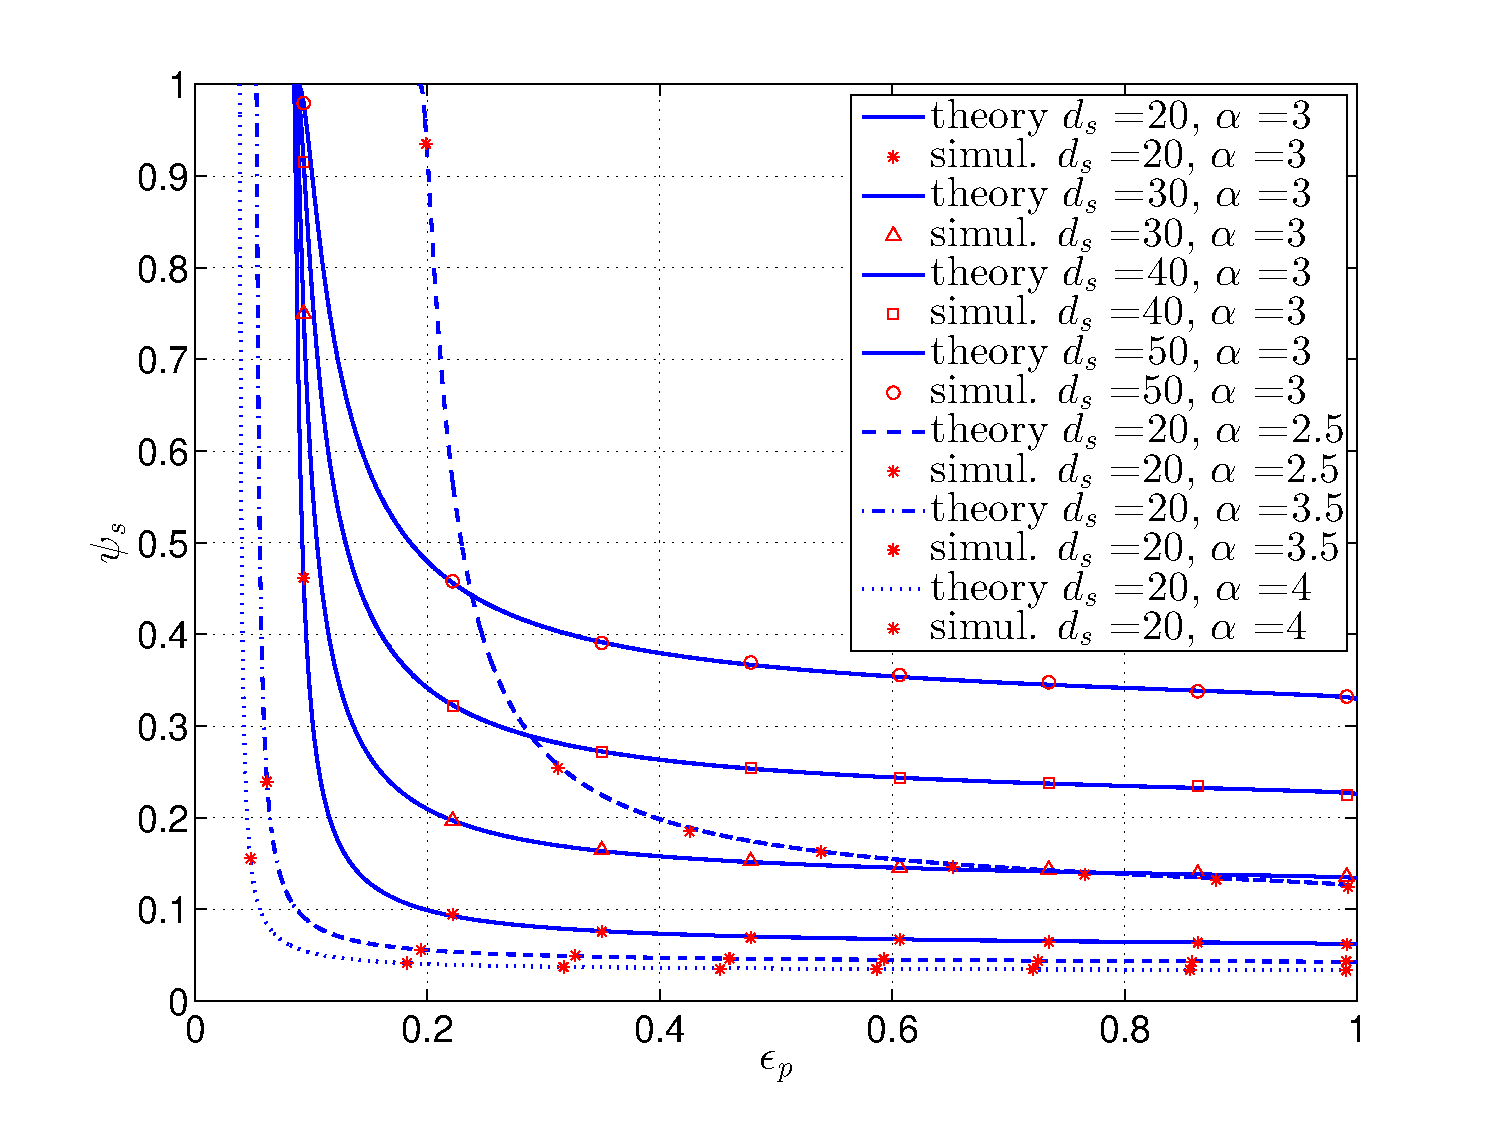
\includegraphics[trim=1.2cm 0.4cm 1.6cm 1.2cm,clip=true,width=\columnwidth]{figures/fig_ID_Cap_Out_vs_epsilon_wkr_1e5.pdf}
        \else
        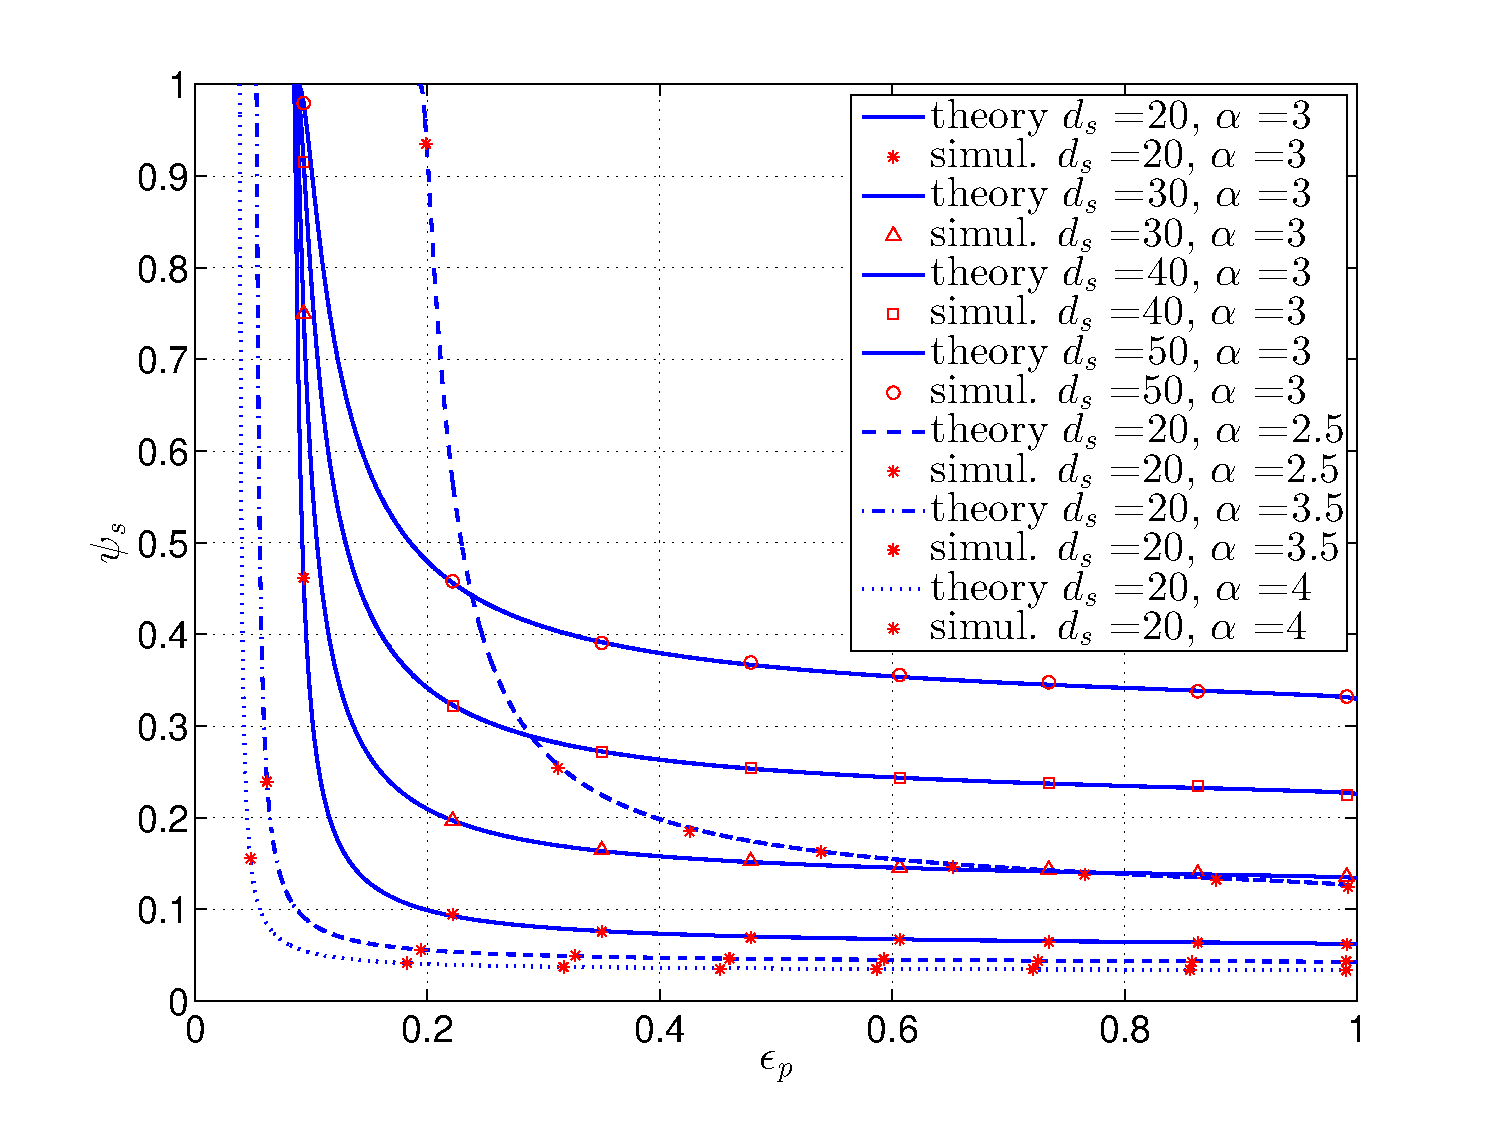
\includegraphics[trim=0.0cm 0.0cm 0.0cm 0.0cm,clip=true,width=0.5 \columnwidth]{figures/fig_ID_Cap_Out_vs_epsilon_wkr_1e5.pdf}
        \fi
\makeatother
\caption{OC illustrating $\mathsf{C}\sub{ID}$ outage $\psi\sub{s}$ at the ID versus the $\mathsf{SIR}\sub{PR}$ outage $\epsilon\sub{p}$ at the PR for the CRN with different choices of $d\sub{s}$ and $\alpha$, where $N\sub{p} = \SI{10}{}$, $R\sub{s} = \SI{2}{bits/sec/Hz}$, $P\sub{p} = \SI{10}{dBm}$, $d\sub{p} = \SI{50}{m}$, $\lambda\sub{p} = 10^{-6} \text{nodes}/{\text{m}^2}$ and $\lambda\sub{s} = 10^{-5} \text{nodes}/{\text{m}^2}$.}
\label{fig:ID_OC}
\end{figure}
%Theorem \ref{th:theo1} presents an expression for the OC. 

OC considers the $\mathsf{SIR}\sub{PR}$ outage probability constraint at the PR $\epsilon\sub{p}$ and the $\mathsf{C}\sub{ID}$ outage probability constraint at the ID $\psi\sub{s}$. 
\begin{remark}
\normalfont
%In (\ref{eq:OC}), $\psi\sub{s}$ decreases with increase in $\epsilon\sub{p}$ and vice versa, with a certain choice of system parameters, refer to \figurename~{\ref{fig:ID_OC}}. 
Again, the expression (\ref{eq:OC}) derived from our system model represents a LPB. Following Remark \ref{rem:rem1}, $\epsilon\sub{p}$ decreases with increase in $\alpha$ and decrease in $d\sub{p}$, which results in a lower $\psi\sub{s}$. Moreover, $m$ in the exponent of (\ref{eq:OC}), decreases proportionally to $\lambda\sub{s}$ and $d\sub{s}^2$, which further lowers $\psi\sub{s}$. Fixing $\theta$, the expression $\ln\left( \kappa/1 - \epsilon\sub{p} \right)$ is held constant, however, $\alpha \sin \left( 2 \pi/\alpha \right)$ increases and $(2^{R\sub{s} - 1})^{\frac{2}{\alpha}}$ decrease with $\alpha$ for $R\sub{s} > 1$, hence, causes a decrease in $\psi\sub{s}$. Thereby, the scenarios with larger $\alpha$, smaller $d\sub{p}$, $d\sub{s}$, e.g., $\alpha \ge 3$, $d\sub{p} \approx \SI{50}{m}$ $d\sub{s} \le \SI{30}{m}$, which attribute to indoor scenarios as illustrated in \cite{Kaushik13}, result in a better OC, cf. \figurename~\ref{fig:ID_OC}. 
\label{rem:rem3}
\end{remark}

To extend the analysis of comparing different scenarios, we consider that the constraint at PR is fulfilled. The performance of the secondary system is investigated based on the first and second moments of $\mathsf{C}\sub{ID}$. The variance $\text{Var} [ \mathsf{C}_{\text{ID}} ]$ may be useful indicator for judging quality of service (QoS) at the ID. 
\begin{coro}
\normalfont
The expected capacity at the ID is given by 
\begin{align}
\e{}{\mathsf{C}_{\text{ID}}} &= \frac{1}{\ln 2} \int\limits_{0}^{\infty} \frac{1}{1+ x} e^{-\mu x^{\frac{2}{\alpha}}} \text{d}x, \label{eq:Exp_Cap}
\end{align}  
where  $\mu = - m \ln \left({1 - \epsilon{\sub{p}}}\right)$ and $\mu \ge 0$. 
%The expression (\ref{eq:Exp_Cap}) obtains an analytical expression. 
For the special case $\alpha = 4$, the following closed-form expression for $\e{}{\mathsf{C}_{\text{ID}}}$ exists 
\begin{align} 
\e{}{\mathsf{C}_{\text{ID}}} &= \frac{1}{\ln 2} \left[ \sin(\mu) \left( \frac{\pi}{2} - \sini(\mu) \right) - \cos(\mu) \cosi(\mu) \right], \label{eq:Exp_Cap_4}  
\end{align}
where $\sini(\cdot)$ and $\cosi(\cdot)$ corresponds to sine and cosine integral \cite{grad}.  
\begin{IEEEproof}
See Appendix.
\end{IEEEproof}
\end{coro}
\begin{coro}
\normalfont
The variance of capacity at the ID is given by 
\begin{align}
\text{Var} [ \mathsf{C}_{\text{ID}} ] &=  \frac{2}{(\ln 2)^2} \int\limits_{0}^{\infty} \frac{\ln(1 + x )}{1 + x} e^{-\mu x^{\frac{2}{\alpha}}} \text{d}x -  {\e{}{\mathsf{C}_{\text{ID}}} }^2. 
\label{eq:var_cap}
\end{align}
%where $\e{}{\mathsf{C}_{\text{ID}}}$ is evaluated in (\ref{eq:Exp_Cap}). 
Similar to $\e{}{\mathsf{C}_{\text{ID}}}$, (\ref{eq:var_cap}) represents the analytical expression for $\text{Var} [ \mathsf{C}_{\text{ID}} ]$. For validation of the theoretical results, $\e{}{\mathsf{C}_{\text{ID}}}$ and $\text{Var} [ \mathsf{C}_{\text{ID}} ]$ are computed numerically and compared with simulations. 
\end{coro}
\begin{figure}[!t]
        \centering
	\makeatletter
	\if@twocolumn
        	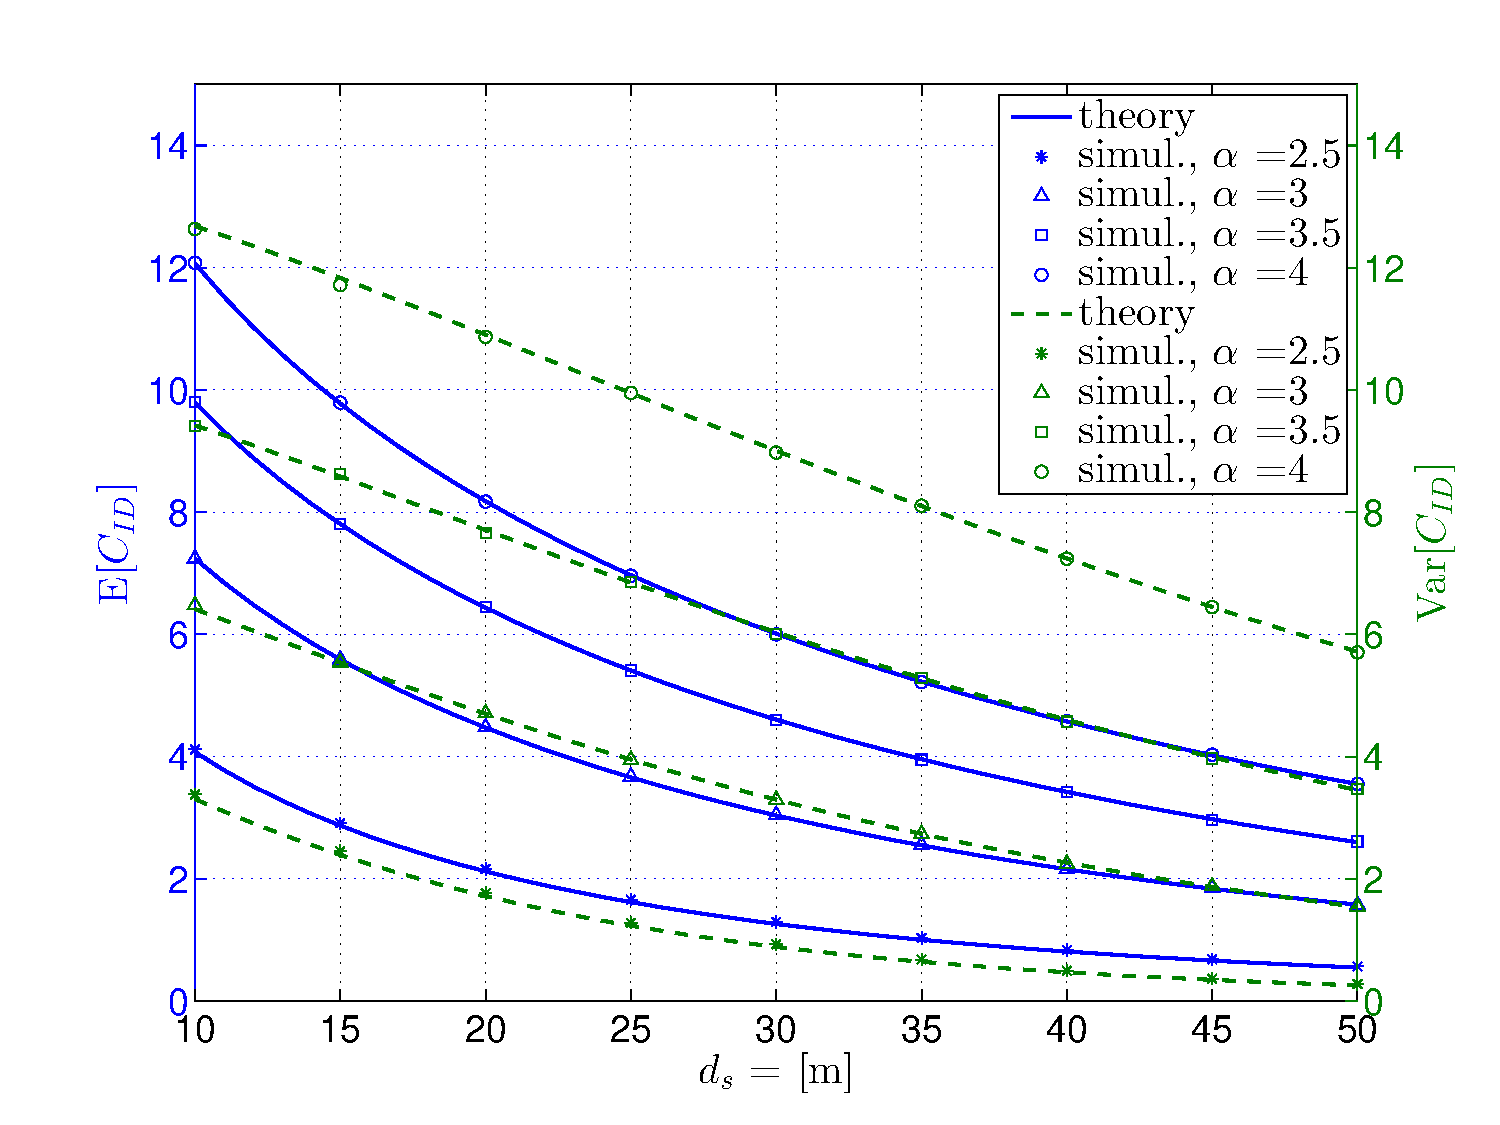
\includegraphics[trim=1.0cm 0.5cm 0.7cm 1.4cm,clip=true,width= \columnwidth]{figures/fig_ID_Cap_Moments_vs_d_s_1e5}
	\else
        	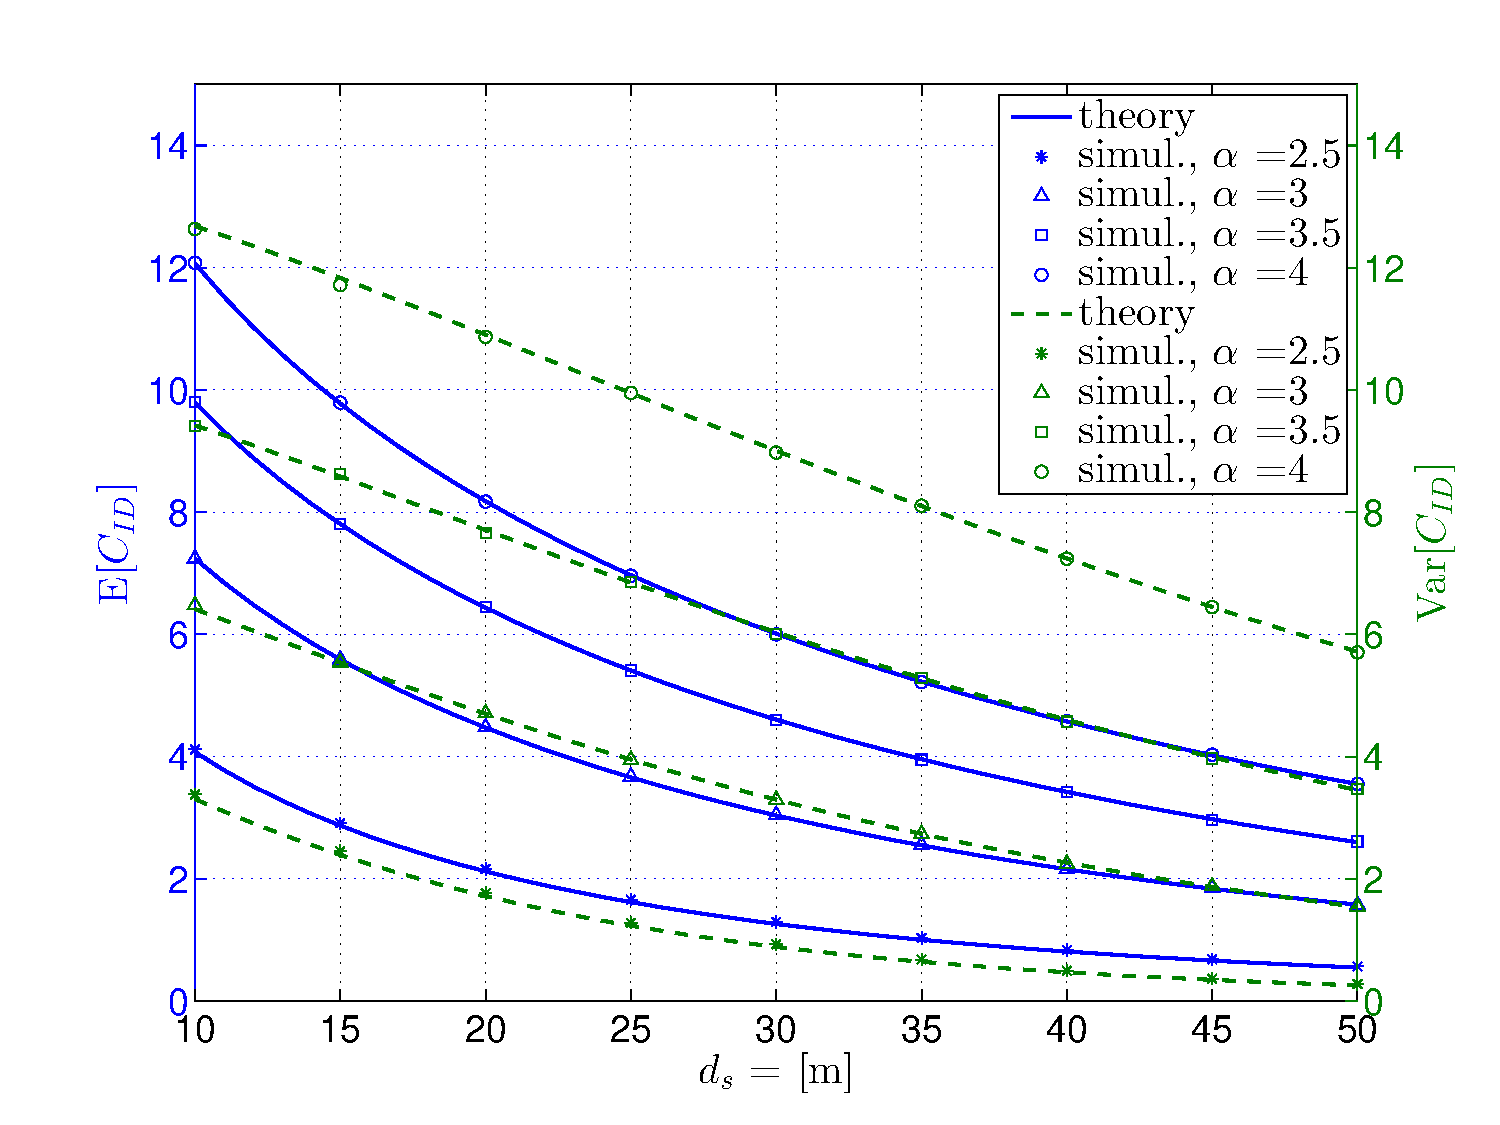
\includegraphics[trim=0.0cm 0.0cm 0.0cm 0.0cm,clip=true,width=0.5 \columnwidth]{figures/fig_ID_Cap_Moments_vs_d_s_1e5}
	\fi
	\makeatother
\caption{$\e{}{\mathsf{C}\sub{ID}}$ and $\text{Var} [\mathsf{C}_{\text{ID}} ]$ of the capacity at the ID against the $d\sub{s}$, after the $\textsf{SIR}\sub{PR}$ constraint is satisfied, with different choices of $\alpha$, where $\theta = 0.95$, $N\sub{p} = \SI{10}{}$ and $P\sub{p} = \SI{10}{dBm}$, $d\sub{p}=\SI{50}{m}$, $\lambda\sub{p} = 10^{-6} \text{nodes}/{\text{m}^2}$, $\lambda\sub{s} = 10^{-5} \text{nodes}/{\text{m}}^2$.}
\label{fig:Cap_Moments}
\end{figure}
%\begin{IEEEproof}
%\normalfont
%To obtain an expression for $\text{Var} [\mathsf{C}_{\text{ID}} ]$, same procedure as used for deriving $\e{}{\mathsf{C}\sub{ID}}$, cf. (\ref{eq:Exp_Cap}), is followed. 
%\end{IEEEproof}
%\begin{remark}
%\normalfont 

$\e{}{\mathsf{C}_{\text{ID}}}$ and $\text{Var} [ \mathsf{C}_{\text{ID}} ]$ depend on the area under $f(x) e^{-\mu x^{\frac{2}{\alpha}}}$, where $f(x)$ is $1/(1 + x)$ and $\ln(1 + x )/(1 + x)$, hence, $f(x)$ is independent of the system parameters. However, rate of decay for the exponential function is controlled by $\mu x^{\frac{2}{\alpha}} = - m \ln({1 - \epsilon\sub{p}})x^{\frac{2}{\alpha}}$. Considering $m$ and following the analysis similar to Remark \ref{rem:rem3}, large $\e{}{\mathsf{C}_{\text{ID}}}$ is obtained for indoor scenarios, cf. \figurename~\ref{fig:Cap_Moments}. However, greater $\text{Var} [ \mathsf{C}_{\text{ID}} ]$ is observed for larger $\alpha$ and smaller $d\sub{s}$, as larger $\alpha$ and smaller $d\sub{s}$ scales the signal and larger $\alpha$ scales the interference from other PTs and CRs of $\mathsf{SIR}\sub{ID}$, cf. (\ref{eq:SIR_ID}). This may influence the QoS at ID. 
%\end{remark}
%%%%%%%%%%%%%%%%%%%%%%%%%%%%%%%%%%%%%%%%%%%%%%%%%%%%%%%%%%%%%%%%%%%%%%%%%%%%%%%%%%%%%%%%%
\section{Conclusion} \label{sec:conc}
%%%%%%%%%%%%%%%%%%%%%%%%%%%%%%%%%%%%%%%%%%%%%%%%%%%%%%%%%%%%%%%%%%%%%%%%%%%%%%%%%%%%%%%%%
The paper provides an extension to the concept of cognitive relay to cognitive relay network. Stochastic geometry is used to model the locations of the primary and secondary systems. The sensing imperfection and model inaccuracies for the cognitive ecosystem decreases the system's reliability. Motivated by this fact, we establish a lower performance bound to benchmark the performance of systems that include model inaccuracies and sensing. Furthermore, we obtain OC to jointly analyze the performance of primary and secondary systems. Based on the OC and the system parameters defined for an indoor scenario, it is indicated that the CRN operating indoor are propitious for the system.
%%%%%%%%%%%%%%%%%%%%%%%%%%%%%%%%%%%%%%%%%%%%%%%%%%%%%%%%%%%%%%%%%%%%%%%%%%%%%%%%%%%%%%%%%
\appendix[Expected capacity at ID]  
%%%%%%%%%%%%%%%%%%%%%%%%%%%%%%%%%%%%%%%%%%%%%%%%%%%%%%%%%%%%%%%%%%%%%%%%%%%%%%%%%%%%%%%%%
\begin{IEEEproof}
\normalfont
Expected capacity for the ID is given as
\begin{equation}
\e{}{\mathsf{C}\sub{ID}} = \int\limits_{0}^{\infty} R\sub{s} \text{d} F_{\mathsf{C}\sub{ID}}(R\sub{s}) \label{eq:Exp_Cap_d1},  
\end{equation}
where $F_{\mathsf{C}\sub{ID}}(R\sub{s})$ is defined in (\ref{eq:OC}). In order to simplify (\ref{eq:OC}), $R\sub{s} = x$, $(1-\epsilon\sub{p}) = b,$ $e = \frac{2}{\alpha}$ is substituted to give
\begin{equation}
F_{\mathsf{C}\sub{ID}}(x) = 1 - b^{\left( 2^{x}-1 \right)^{e} m } = 1 - c^{\left( 2^{x}-1 \right)^{e}}, \label{eq:Exp_Cap_d3}  
\end{equation}
where $c = b^m$. Using (\ref{eq:Exp_Cap_d3}) to evaluate (\ref{eq:Exp_Cap_d1}) yields 
\begin{equation}
\e{}{\mathsf{C}\sub{ID}} = \ln 2 \cdot \ln c \int\limits_{0}^{\infty} x e 2^x (2^x - 1)^{e-1} c^{(2^x - 1)^e} \text{d}x. \label{eq:Exp_Cap_d4} \\
\end{equation}
%\intertext{Substituting $2^x - 1 = y$ and applying product rule gives the general expression for expected capacity (\ref{eq:Exp_Cap})}
%\quad &=  \frac{1}{\ln(2)} \int\limits_{0}^{\infty} \frac{1}{y + 1} e^{-\mu y^e} \text{d}y, \label{eq:Exp_Cap_d4}  
Solving (\ref{eq:Exp_Cap_d4}) obtains the general expression for the expected capacity (\ref{eq:Exp_Cap}), where $\ln({1}/{c}) = \mu$. For $\alpha = 4$, (\ref{eq:Exp_Cap_d4}) gives
\begin{equation}
\e{}{\mathsf{C}\sub{ID}} = \frac{1}{\ln 2} \int\limits_{0}^{\infty} \frac{2x}{x^2 + 1} e^{-\mu x} \text{d}x. \label{eq:Exp_Cap_d5}  
\end{equation}
Applying \cite[3.354]{grad} to (\ref{eq:Exp_Cap_d5}) yields (\ref{eq:Exp_Cap_4}).
\end{IEEEproof}


%%%%%%%%%%%%%%%%%%%%%%%%%%%%%%%%%%%%%%%%%%%%%%%%%%%%%%%%%%%%%%%%%%%%%%%%%%%%%%%%%%%%%%%%%
% References
%%%%%%%%%%%%%%%%%%%%%%%%%%%%%%%%%%%%%%%%%%%%%%%%%%%%%%%%%%%%%%%%%%%%%%%%%%%%%%%%%%%%%%%%%
\bibliographystyle{IEEEtran}
\bibliography{IEEEabrv,refs}

% that's all from my side 
\end{document}
